\documentclass[12pt,a4paper,english
% ,twoside,openright
]{tunithesis}

% Note that you must choose either Finnish or English here and there in this
% file.
% Other options for document class
  % ,twoside,openright   % If printing on both sides (>80 pages)
  % ,twocolumn           % Can be used in lab reports, not in theses

% Ensure the correct Pdf size (not needed in all environments)
\special{papersize=210mm,297mm}


% LaTeX file for BSC/MSc theses and lab reports.
% Requires the class file (=template) tunithesis.cls and figure files,
% either tut-logo, exampleFig (as pdf or eps) and example_code.c
% Author: Lucas Machado (2018)
% Based on TTU template by Sami Paavilainen (2006), modified by Heikki Huttunen (2014)


% More information about Latex basics:
% [Tobias Oetiker, Hubert Partl, Irene Hyna, Elisabeth Schlegl, The
% Not So Short Introduction to LATEX2e, Version 5.03, April 2014, 171
% pages.  Availbale: http://tobi.oetiker.ch/lshort/lshort.pdf]


%
% Define your basic information
%
\author{Chen Zhu}
\title{A Machine Learning Approach of Logistic Organ Dysfunction Score Estimation with Data Acquired from Bedside in ICU} % primary title (for front page)
\thesistype{Master's thesis} % or Bachelor of Science, Laboratory Report... 

% Put your thesis' main language last
% http://mirrors.ctan.org/macros/latex/required/babel/base/babel.pdf
\usepackage{lastpage}
\usepackage{comment}
\usepackage{multirow}
\usepackage[english]{babel}
\usepackage[
backend=biber,
style=authoryear,
citestyle=authoryear,
autocite=inline
]{biblatex}
\usepackage{csquotes}
\usepackage{lscape} 
\usepackage{threeparttable}
\usepackage{amsfonts}

\addbibresource{thesis_refs.bib} %Imports bibliography file

%
% You can include special packages or define new commands here at the
% beginning. Options are given in brackets and package name is in
% braces:  \usepackage{opt]{pkg_name}

% Option1) for bibliography does not need additional packages.

% Option2b) for bibliography: old way for using Name-year citations
% http://www.ctan.org/tex-archive/macros/latex/contrib/harvard/ 
%\usepackage{harvard}  


% Option3) for bibliography: newer way, esp. for Name-year citations
% http://www.ctan.org/pkg/biblatex
%\usepackage[style=authoryear,maxcitenames=2,backend=bibtex,
%  firstinits=true]{biblatex}
%% Note that option style=numeric works as well
%\addbibresource{thesis_refs.bib}

\definecolor{tunipurple}{RGB}{78, 0, 142}

% You can also add your own commands
\newcommand\todo[1]{{\color{red}!!!TODO: #1}} % Remark text in braces appears in red
\newcommand{\angs}{\textsl{\AA}}              % , e.g. slanted symbol for Ångstöm
\renewcommand{\thetable}{\arabic{table}}
% Preparatory content ends here



\pagenumbering{roman} % was: {Roman}
\pagestyle{headings}
\begin{document}



% Special trick so that internal macros (denoted with @ in their name)
% can be used outside the cls file (e.g. \@author)
\makeatletter



%
% Create the title page.
% First the logo. Check its language.
\thispagestyle{empty}
\vspace*{-.5cm}\noindent

\begin{figure}
    \vspace{-1.3cm}
    \advance\leftskip-2.5cm
    \noindent
\includegraphics{img/tunilogo.png}
\end{figure}
 
\vspace{2.5cm}
\begin{flushright}
\noindent\textsf{\LARGE{\@author}}

\noindent\vspace{0.5cm}

\noindent\Huge{\textsf{\textbf{\textcolor{tunipurple}{\@title}}}}
\end{flushright}
\vspace{10.7cm} % adjust to 12.7 this if thesis title needs two lines

% Last some additional info to the bottom-right corner
\begin{flushright}  
    \begin{spacing}{1.0}
      \textsf{Faculty of Information Technology and Communication Sciences (ITC)\\
      \@thesistype\\
      April 2024}
    \end{spacing}
\end{flushright}

% Leave the backside of title page empty in twoside mode
\if@twoside
\clearpage
\fi

% Turn off page numbering for the first pages
\pagenumbering{gobble}


% Some fields in abstract are automated, namely those with \@ (author,
% title, thesis type).

\chapter*{Abstract}

\begin{spacing}{1.0}
\noindent \@author: \@title\\
\@thesistype\\
Tampere University\\
Master’s Degree Programme in Software Development\\
April 2019
\end{spacing}
\noindent\rule{12cm}{0.4pt}

\vspace{0.5cm}

% ---------------------------------------
% Abstract and keywords
% ---------------------------------------

\noindent Intensive Care Unit (ICU) is a high-stakes environment in hospital, where patients are in higher danger than other departments, for instance organ dysfunction, and monitored with devices and more care worker. Effectively predicting patient status in an ICU is a critical task serving patient health and resource allocation Logistic Organ Dysfunction Scale (LODS), with weighted variables with the worst values in first 24h, is an organ dysfunction score system which reflects severity level within an organ system and among organ systems. It is considered as an outcome risk prediction scoring system as well, since an equation is included that converts LODS into probability of mortality. It is confirmed to be usable for the first 7 days in ICU, and is widely used in other departments as well. LODS calculation needs some laboratory results, such as bilirubin, which cost time and money. Effective prediction of LODS value could measure patient overall organ dysfunction situation and calculate probability of mortality for patient.
\noindent There are a little researches predict LODS with both laboratory result and bedside data. This thesis is to propose machine learning models, trained with XGBoost and Convolutional Neural Network, whose training dataset is the Medical Information Mart for Intensive Care (MIMIC) -IV database, to predict total LODS with data that can be acquired from bedside in first 12 hours of ICU stay, to save time and assist doctor in treatment. 




~

\noindent\textbf{Keywords:} machine learning, organ dysfunction score.

~

\noindent The originality of this thesis has been checked using the Turnitin Originality Check service.


% Add the table of contents


\setcounter{tocdepth}{3}              % How many header level are included
\tableofcontents                      % Create TOC


% The actual text begins here and page numbering changes to 1,2...
% Leave the backside of title empty in twoside mode
\if@twoside
%\newpage
\cleardoublepage
\fi


\renewcommand{\chaptername}{} % This disables the prefix 'Chapter' or
                              % 'Luku' in page headers (in 'twoside'
                              % mode)


\chapter{Introduction}
\label{ch:intro} 

\pagenumbering{arabic}
\setcounter{page}{1} % Start numbering from zero because command
                     % 'chapter*' does page break
                     
% \label{...} allows cross-referencing, e.g. 'as explained in
% Chapter~\ref{ch:intro}' Note that you may have to run the command
% 'latex' or 'pdflatex' twice to get cross-references correctly.  You
% can add labels e.g. to chapters, sections, figures, tables, and
% equations.

% You can write everything into single tex file. Alternatively, you
% can write each chapter into separate file and then include them her
% \include{intro} % no postfix .tex to the command
% \include{related_works} % and so on...

Since the first intensive care unit (ICU) established in Denmark in 1953, the ICU has become an essential element in hospital-care based health care. An intensive care unit is defined as an organized system to treat critically ill patients with intensive and specialized medical and nursing care, an enhanced capacity for monitoring, and multiple methods of physiologic organ support to sustain life when patient has acute organ system insufficiency. An ICU's activities are not limited to the geographic area in a hospital, but extend to include emergency department , hospital ward and follow-up clinic. \parencite{Marshell2017} Patients with critical illness might be found throughout a hospital, however, many of them are treated in ICU. ICU mortality varies by different conditions, for instance, according to \textcite{Adhikari2010}, 8-18\% in unselected patients in North America, Europe, Australia, and New Zealand, 35–45\%48 in heterogeneous cohorts of patients with acute lung injury, and 50–60\%49 in patients with septic shock. Patients in ICU are in three main categories: those with acute organ dysfunction (including those who receives long-term intensive organ support because of their unclear ultimate outcome), those who had a major procedure and are monitored in the peri-intervention period, and those who are receiving end-of-life care. To give sufficient but not excessive treatment, ICU is divided into different levels. A level 1 provides oxygen, noninvasive monitoring, and more intensive nursing care than on a normal ward, where a level 2 ICU is capable to provide invasive monitoring and basic life support for a short period. A level 3 ICU serves as a regional resource for critically ill patients by providing a full spectrum of monitoring and life support technologies. It may play an active role in developing the specialty of intensive care through research and education. \parencite{Marshell2017} Patients, families and care providers concern recovery likelihood, however, prognostication can be difficult in ICU. Scoring systems are used to objectively quantify condition severity and risk stratify patients for prognostication in clinical. They are also used as standard tools in critical care research to demonstrate equivalence of patients group. \parencite{Tiffany21}

Scoring systems are tools used in critical care to clinically objectively quantify severity, risk stratify patients for clinical prognostication and in research as study inclusion criteria and to demonstrate equivalence of patient groups. It can broadly be divided into those that are specific for a disease or an organ, for example the Glasgow Coma Scale, and those that are for all ICU patients. The scores that are generic for all ICU patients are broadly divided into: 1) scores that assess severity on admission and predict outcome, for example, Acute Physiology and Chronic Health Evaluation (APACHE), 2) scores that assess the severity of organ dysfunction, for example, Sequential Organ Failure Assessment (SOFA), 3) scores that assess nursing workload using, for example, Nine Equivalents of Nursing Manpower Use Score (NEMS). \parencite{Tiffany21, Jonathan2008, Rapsang2014, Vincent2010} Logistic Organ Dysfunction Score \parencite{legall96}, as somewhere between mortality prediction score and organ dysfunction score, is developed to assess and characterize current degree of organ dysfunction. \parencite{Tiffany21, Vincent2010} It selects 12 variables to represent the function of six organ systems, which include laboratory results and non-invasive parameters. It ranges from 0 to 22 where 0 is no dysfunction and 22 is maximum dysfunction. It also included a logistic regression equation that can convert the score into a probability of mortality. Although it was not initially validated for repeated use in ICU, \textcite{Timsit2002} validated that LODS characterized the progression of organ dysfunction accurately in the first 7 days of ICU stay.

Machine learning is a branch of artificial intelligence, broadly defined as the capability of a machine to imitate the way that human learns. It is the foundation behind predictive text, language translation apps, and the way social media feeds are presented. \parencite{sara2021} Quoted to \textcite{samuel1959}, machine learning is that computers can be given the ability to learn without being explicitly programmed. What this means is that a computer program learns with observed data and a learning algorithm to perform a task, such as predicting result. Generally, data in machine learning is split to two groups, a training set and a test set. As the name suggests, the training set is used to train algorithm where features are included. The test set is used to algorithm performance and it is new to the algorithm. Once an algorithm passes the training and test phases with an acceptable performance, it will be implemented to real world. The adoption of machine learning can be found in science, commerce and technology, including the diagnosis of faults in complex systems and consumer services. \parencite{jorden2015} In healthcare, machine learning has evolved for years. It is capable to assist case triage, enhance image scanning and segmentation, and support decision making, and it has changed and will shift healthcare epidemiology, for example, predicting risk of Nosocomial Clostridium difficile Infection (CDI) and predicting clinical outcomes in Ebola Virus Disease (EVD) Infection using initial clinical symptoms. \parencite{Jenna2017, Habehh2021} In addition, machine learning is applied a lot in electronic health records (for example, analys heart failure survival \parencite{Panahiazar2015}), medical imaging (for example, detecting diabetic retinopathy from retinal photographs \parencite{Gulshan2016}), and genetic engineering (for example, predicting the immunogenic landscape of SARS-CoV-2 \parencite{Malone2020} ).

Medical score system needs accuracy to reflect patients’ condition, and ease of use to reduce clinician time in using and learning. Only if a score system is substantially better than another one, proved by a large number of research, it will be used in practice. So improving an existed score system is more feasible than replacing, and change should be small but useful. LODS esitmates with the worst value of the first 24 hours of ICU stay, both bedside and laboratory measurements, which cost money and time. This research would use only bedside data because they are easy to access, without long-time waiting or money cost. And for some dangerous patients, 24 hours is a long time to collect data. If 24h severity can be predicted early, doctors will be able to change the treatment. LODS is a hybrid scoring system which makes it a good tool in this prediction. As human physiology comprises a complex system, using mathematical models to analyse organ dysfunction may describe systemic host response to infection or injury. \parencite{seely2011} So in this research, machine learning is brought to bedside to predict patients' severity by predicting LODS. ICU has many monitoring devices and produces a large amount lab test results which is a great resource for machine learning model training and research.

XGBoost algorithm is used for predicting part in this study, supported by \textcite{xgboost_lib}. Convolutional Neural Network is used for feature engineering in some models, supported by TensorFlow library. Some vitals signs, include heart rate, respiratory rate, Systolic blood pressure(sbp), Diastolic blood pressure (dbp), mean arterial pressure (MAP), Oxygen Saturation (SPO2), and temperature in the first 12 hours of ICU stay, and other bed side data, include GCS, GCS eye, GCS motor,the total urine output in the first 12 hours, and the most mechanical ventilation method are taken as input to the models, and output is the total LODS value in the first 24h ICU stay. The target is to check if predicting total LODS value to represent patient's 24h situation with 12h bed side data is possible and practicable.

This document is structured as follow. Chapter ~\ref{ch:background} shows the basic organ dysfunction scoring system and machine learning concept. Chapter ~\ref{ch:priorwork} shows some prior related research, mostly about predicting and evaluating patients' situation with bed side data. Chapter ~\ref{ch:methods} introduces the data source and the algorithms used in this study. Chapter ~\ref{ch:experiment} shows the experiments' details and results, and chapter ~\ref{ch:conclusion} discusses the result and shortcomings of this study and some further research direction.


\chapter{Background}
\label{ch:background}
This chapter aims to show the concept of severity scoring system in critical care and introduce the scoring system, Logistic Organ Dysfunction Score, used in this study. The concept of machine learning is also introduced in this chapter to give a brief idea about machine learning.

\section{Severity Scoring systems in Critical Care}
ICU is one of the most dangerous department in a hospital, where patients situation varies but in serious condition. In critical care, physiology-based scoring systems applied much more than diagnosed-based scoring systems, because sometimes no diagnoses are made on admission and patients in ICU can have more than one organ failure where diagnose-based scoring system is inapplicable. \parencite{Bouch2008} Severity scores are divided into those calculated with data obtained in the first day of ICU admission (for example, the mortality prediction model (MPM)), and those calculated with data collected sequentially throughout the duration of ICU stays (for example, the Sequential Organ Function Assessment (SOFA)). 

Both first day and sequential systems can be divided into subjective scores and objective scores. Subjective scores are established by taking variables and applying weights on them based on personal experience of a panel of experts. A range of normality is defined for each variable. The higher weights are assigned to more abnormal results, mostly from 0 to 4. The final score is the total number of points. For instance, Sequential Organ Failure Assesssment (SOFA). Objective scores are developed from a large database of clinical data which is compiled from many ICUs. A multipurpose probability model will be applied to determine ranges, assign weights, and select variables. Variables can be classified into four groups: age, comorbidities, physiological abnormalities, and acute diagnoses. Outcome of these systems are on vital status at hospital discharge predominantly and other measures (for example, life among long-term survivors and vital status 28 days after hospital discharge or quality). All systems result in a logistic regression model to estimate or assist in estimating the risk of death. \parencite{LeGall2005, Bouch2008} 

The principle use of severity scoring systems is to predict and evaluate individual patient's situation. Outcome prediction scores and organ dysfunction are two main categories of severity scoring system, which are respectively used to objectively predict risk of death and assess organ dysfunction. Outcome prediction score was originally developed to provide an indication of the risk of death of groups of ICU patients. However, with the development of medical data and practice, include patient demographics, disease prevalence, and intensive care practice, and statistical and computational techniques, the updated versions of those scores can be applied to individual patient. For instance, the four versions of Acute Physiology and Chronic Health Evaluation (APACHE)  are widely used in ICUs worldwide. Organ dysfunction scores are primarily designed to describe the degree of organ dysfunction. The severity of organ dysfunction varies from one individual patient to another and over time for one individual. Organ dysfunction should take both time and severity into account. There is not a score that covers all organ systems. Moreover, for all organ systems that one score covers, accuracy might varies. \parencite{LeGall2005, Bouch2008, Vincent2010} Severity score systems give assistance in clinical decisions by its objectivity, although they are not always accurate. It's prudent to use severity systems in decision-making, instead of only subjective opinion. But according to \textcite{LeGall2005, Vincent2010-at}, severity scores should not be used to dictate individual patient decisions. In addition, severity scores are also used in clinical trial (for example, evaluating how organ dysfunction affects sepsis morbidity), and evaluation of ICU performance (for example, comparing the probabilities of hospital mortality and actual outcome in ICUs in several countries). \parencite{LeGall2005, Vincent2010}

This research focus on Logistic Organ Dysfunction Score, an organ dysfunction score which is originally designed for first-day use in ICU. When compare with other scores, it can also be used to calculate probability of mortality with an equation, and it has simple calculation. It is a score that can be used for two purposes. So predicting LODS can be considered as predicting organ dysfunction situation and probability of mortality together. 

\subsection{Logistic Organ Dysfunction Score}
Logistic Organ Dysfunction Score, acronym as LODS, is initially proposed by \textcite{legall96}. The initial goal was to propose an objective system that can reflect  patient severity adequately, and as simple as possible to apply.  In many scoring systems, each organ system is graded from 1 to 4 or from 1 to 6, which are different from the ranges found using statistical methods. Moreover, all organ systems are weighing in the same way does not take the differential prognostic significance of the involved organs into account. 

LODS was proposed with the large database of the European-North American study (ENAS), where 14,745 consecutive admissions in 137 medical, surgical, or mixed ICUs in 12 countries. Only patients aged 18 years or older were eligible; burn patients, coronary care patients, and cardiac surgery patients were excluded. Twelve variables were selected by multiple logistic regression to represent the function of six organ systems (neurologic, cardiovascular, renal, pulmonary, hematologic, hepatic). The worst value for each variable within 24 hours of ICU admission are ranked to a scale that considers no dysfunction with 0 to maximum dysfunction with 5. LODS is a weighted system: the maximum score allowed for the respiratory and coagulation is 3, and the maximum score for liver is 1. Therefore, LODS value ranges from 0 to 22, as Table \ref{table:lods}. For sedated patients, the GCS was ascertained either by reviewing the patients' medical record before sedation, or from interviewing the physician who ordered sedation. A variable was assumed to be normal if it was not measured. All variables were continuously scaled except platelet count and prothrombin time. The worst value of first 24h refers to the worst recorded values that received the highest number of LOD points. For example, if a patient at different has tachycardia of 150 beats per minute (1 LOD point) and bradycardia of 25 beats per minute (5 LOD points), 5 is recorded for cardiology. LODS is considered as a hybrid organ dysfunction and outcome risk prediction scoring system as it combines a global score summarizing the total degree of organ dysfunction of the organ systems, and a logistic regression equation that can convert the score to a probability of mortality (e indicated to a mathematical constant 2.7182818). Within organ systems, higher mortality is associated with greater severity scores, that a LODS of 22 is associated with a mortality of 99.7\%. \parencite{Tiffany21, Vincent2010, sekulic2015}

\begin{equation*}
Predicted Death Rate = (e^{-3.4043 + 0.4173*(LODS)} ) / ( 1 +  e^{-3.4043 + 0.4173*(LODS)} )
\end{equation*}

LODS was originally developed for the first 24 hours of ICU stay, but it is also validated as an accurate organ dysfunction score in the first 7 days of ICU stay by \textcite{Timsit2002} in a study of 1,685 patients in French ICUs. \textcite{Metnitz2001} confirmed that LODS is well correlated with the numbers and levels of dysfunctions, and well in discriminating survivors and non-survivors in a study with 2893 consecutive admissions in ICU in Austria, from which LODS was considered to provide combined measure of morbidity and mortality for patients critically ill with multiple organ dysfunction/failure. \textcite{Blanco2008}  proved that total LODS score was associated with early death of patients with severe sepsis in ICU.


\begin{landscape}
    \begin{table}[]
    \begin{threeparttable}
        \caption{Logistic Organ Dysfunction Score.}
        \label{table:lods}
        \begin{tabular}{lllllllll}
            \hline
            \textbf{Organ system} & \textbf{Parameter} & \textbf{5} & \textbf{3} & \textbf{1} & \textbf{0} & \textbf{1} & \textbf{3} & \textbf{5} \\
            \hline
            Neurologic & GCS\tnote{1} & 3-5 & 6-8 & 9-13 & 14-15 & - & - & - \\
            Cardiologic & HR\tnote{2} (beats/min) & \textless 30 & - & - & 30-139 & 140 & - & - \\
             &  &  & or &  &  & and & or &  \\
             & SBP\tnote{3} (mmHg) & \textless 40 & 40-69 & 70-89 & 90-239 & 240-269 & $\geq$270 & - \\
            Renal & Urea nitrogen (mmol/l) & - & - & - & \textless{}6 & 6-9.9 & 10-19.9 & $\geq$20 $\geq$ 1.20 \\
             & (g/l) &  &  &  & \textless{}0.36 & 0.36-0.59 & 0.60-1.19 &  \\
             &  &  &  & and & or & or &  &  \\
             & Creatinine ($\mu$mol/l) & - & - & - & \textless{}106 & 106-140 & $\geq$141 & - \\
             & (mg/dl) &  &  &  & \textless{}1.20 & 1.20-1.59 & $\geq$1.60 &  \\
             &  &  &  & and &  & or &  &  \\
             & Urine output (l) & \textless{}0.5 & 0.5-0.74 & - & 0.75-9.99 & - & \textgreater{}=10 &  \\
            Pulmonary & PaO2 mmHg/FiO2 (on MV or CPAP) &  & \textless{}150 & $\geq$150 & no MV no CPAP & - & - & - \\
             & PaO2 kPa/FiO2 & - & \textless{}19.9 & $\geq$19.9 & no IPAP & - & - & - \\
            Hepatic & Bilirubin ($\mu$mol/l) & - & - & - & \textless{}34.2 & $\geq$34.2 & - & - \\
             & (mg/dl) &  &  &  & \textless{}2.0 & $\geq$2.0 &  &  \\
             &  &  &  &  & and & or &  &  \\
             & PT\tnote{4}time (secs) & - & - & - & $\leq$3 & \textgreater{}3 & - & - \\
             & above standard (\%) &  &  & \textless{}25 & 25 &  &  &  \\
            Hematologic & Leukocytes (× 10 9/l) & - & \textless{}1.0 & 1.0-2.4 & 2.5-49.9 & $\geq$50.0 & - & - \\
             &  &  &  & or & and &  &  &  \\
             & Platelets (109/l) & - & - & - & \textless{}50 & \textgreater{}=50 &  &  \\
             \hline
        \end{tabular}
        \begin{tablenotes}
            \item[1] GCS: Glasgow coma scale; 
            \item[2] HR: heart rate; 
            \item[3] SBP: systolic blood pressure;        
            \item[4] PT: prothrombin
        \end{tablenotes}
        \end{threeparttable}
    \end{table}
\end{landscape}


\section{Machine Learning}
Machine learning is usually divided into three types, 1) supervised training whose goal is to learn mapping from inputs to outputs, 2) unsupervised training whose goal is to find "interesting pattern" in the input data, 3) and reinforcement learning which is useful in learning how to give reward and punishment. In this thesis, we will focus on supervised training. Two most common categories of supervised training are classification and regression. Classification is widely used when outputs are categorical, such as Male and Female. Labels and outputs in regression are finitely discrete and continuous, respectively, such as the age a viewer of a video in YouTube. In this thesis, we focus on mapping measurements of patients’ situation to the LODS value. Typically, the measurements are referred to as features, while the LODS are referred to the target variable. Besides algorithm and model, training process also needs a notion called loss. In most cases, the machine learning tries to minimise the loss between expectation and real target in the training dataset. However, the objective of a model is not performing well in the training set, but in the unseen data. Generally, to archive this target, a three-way split is performed on the dataset, training set, validation set and test set. The goal is to maximise the performance of model in the test set. The main use of validation set is to choose the hyperparameters of the model, which are not optimized by the learning algorithm. Regularisation parameter is an important class of hyperparamenter to control under-fitting and over-fitting on training set. Under-fitting refers to that model learns too crude between predictors and targets, while overfitting refers to learning too complex. Both situation can be diagnosed by comparing training error and validation error. Underfitting is associated with high error in both training and validation, while overfitting is associated with low error in training but high error in validation. Both situation will cause high error in test set which is called generalisation error. Regularisation aims to balance the underfitting and over fitting. Bias and variance are widely checked in regression. Bias checks if the parameters entered the true parameters, and variance checks the spread level of the parameters. Both are inevitable, so the target is to balance the bias and variance to get an optimal model.
Another way to choose hyper parameter is to perform cross validation. A common form of cross validation is K-fold validation. Instead of a single training and validation set, K folds training and validation sets are formed by partitioning the available dataset. Each set is used as validation set at a time and others are used as training set. At the end, the averaged validation error is obtained to monitor the training performance. 



\chapter{Prior Work}
\label{ch:priorwork}
Machine learning has been brought to ICU severity prediction and estimation in many research, with different prediction targets, different data and different algorithms. In this chapter, our intention is to highlight some prior work on three categories that we deemed relevant. First, we focus on the existed research related to prediction models using bed side data at ICUs, and we will also discuss a research which is similar to one experiment of this thesis in this section. Second, we check the works the use of LODS and SOFA, which is another organ dysfunction score, as target or part of the model. There is one example directly connected to the research of this thesis. Finally, we will explore the use of Convolutional Neural Network and XGBoost in medical related machine learning models. 

\section{Models with bed side data in ICU}
In this section, we provide a literature survey of using bed side data in ICU related prediction models, includes pediatric ICU. Electronic Health Record (EHR) is widely used in previous efforts to predict health outcomes, which it contains static or slowly evolving information, medical notes, laboratory test information, etc. However, few studies focused on bed side data, which comes from monitors. Instead of an extensive review of the studies, we will focus on data process, feature extraction and results.

\textcite{mitdavid2020} conducted a study on prediction of length of stay after intubation with continuous vital sign information and static clinical data. The authors uses vital signs from the Medical-Surgical ICU at Boston Children's Hospital, collected by routine bedside monitors (Philips IntelliVue MP90, Philips, Andover, Massachusetts) and recorded with a 5-s frequency by using the T3 system (Etiometry, Allston, Massachusetts), include heart rate, breathing frequency, pulse and SPO2, and some static clinical data to conduct the study. Gaussian processes was applied for missing data imputation to close gaps $\leq$ 20 minutes in vital signs at a given point, as it systematically calculates the imputed data without any structural assumption. The raw time series data from monitors are converted into vectors of statistical features with feature-based methods, and then a clustering strategies based unsupervised learning approach was applied to select features.

Three classification studies were designed, 1) using vital sign information only to classify, 2) using static clinical data only to classify, and 3) using both time series vital signs and static clinical data to classify. After comparison, the 3rd scenario got the best performance that area under the curve of 0.9, 95\% CI [0.80-0.96] which is better than other models to perform a similar task, while using static clinical data only got 0.73 and using vital sign information only got 0.83.

In \textcite{horton2022}, William and others show a predictive model of impending ICU hypoglycemia. This study was conducted with patients' data of ICU admissions at the University of Virginia Medical Center from October 2013 to August 2017. The patients involved were those who were greater than 18 years old and received insulin therapy. William and others took hypoglycemia as the primary outcome, which is defined as any episode of blood glucose less than 70 mg/dL and 50\% dextrose injection was administered within 1 hour. There are 61 vital signs, laboratory values, demographics, and continuous cardiorespiratory monitoring variables, include respiratory rate measured by pulse oximetry and chest impedance, systolic blood pressure by cuff measurement, are selected to perform the univariable analysis and 41 measurements are used in multivariable modeling. After removing the most predictable features correlated more than \textit{R}2 of 0.9 with other features and imputing the missing data with median values, a model with logistic regression was built. A 10 fold cross validation was applied. 

The cross-validated AUROC of the model  was 0.83, which is higher than models consisting of laboratory values only (excluding glucose), vital signs only, and continuous monitoring variables only. Moreover, this study also performed an external validation in the Medical Information Mart for Intensive Care (MIMIC-III) Waveform Database Matched Subset, which contains 22,317 waveform records and 22,247 numeric records for 10,282 distinct ICU patients at the Beth Israel Deaconess Medical Center, and got a good result that AUROC is 0.79

\textcite{yijing2022} proposed a real-time and interpretable model with bedside vital signs monitoring to predict cardiac arrest in critically ill patients. The model was trained with the Medical Information Mart for Intensive Care (MIMIC-III) database. Four vital signs are collected with multi-parameter waveform data, includes electrocardiogram (ECG), SpO2, invasive blood pressure (IBP) and respiratory (RESP) waveform data. Interquartile range was applied to identify outliers, that values outside of Q1 and Q3 are considered as outliers. Then the missing measurements were imputed with carry-forward imputation. The preprocessed vital signs, include HR, systolic blood pressure (SBP), diastolic blood pressure (DBP), mean blood pressure (MAP), SpO2 and RR, are adopted as raw features of the model, and conducted to 43 features. XGBoost algorithm was used to train the model, together with three fold cross validation. The authors also used Shapley Additive exPlanations (SHAP) values to quantify the impact of each feature. As a result, the model successfully identified 95\% cardiac arrest patients, and 80\% of cardiac arrest patients were detected 25 minutes before the event happens. However, it also has error rate 37\% in non cardiac arrest patients, with an overall accuracy of 66\%.

\textcite{gultepe2013} used three vital signs, temperature, respiration rate and mean arterial pressure, and white blood count (WBC) to propose models for lactate level prediction for people with sepsis. The research used records of 741 patients for whom all seven variables were available from EHR of University of California Davis Health System, 590 of which were non-sepsis controls and 151 were with sepsis. It took the the vital signs and WBC as input and lactate level for each patient as target. The cut-off point of lactate level is set to 4 mmol/L that high lactate level is higher than 4mmol/L and low level is lower that it. The prediction was performed with the classification algorithms of Naive Bayes (NB) and clustering using Gaussian Mixture Model (GMM), and Hidden Markov Model (HMM). As a result, the prediction performed well in the second 24 hour time. The GMM classifier had the highest mean AUC (µGMM=0.794, µHMM=0.709, µNB=0.664; all comparisons p<0.05) shown from the Tukey post hoc test. This research also has another part about use the predict mortality risk for patients with sepsis. It demonstrates the feasibility of using Support vector machines (SVM) classification with feature selection for the prediction with only three variables, median lactate levels, median mean arterial pressure, mean absolute deviation of respiration rate. The accuracy is 0.73 which is comparable with another model with more complicated variables.

\section{Organ dysfunction score involved}
This section will show literature review of studies that involved organ dysfunction scores. As this study focuses on machine learning, we will only select studies that cover machine learning, ICU for adults and organ dysfunction scores. In the first two reviews, we focus on how the organ dysfunction score are involved. In the last we will review the whole study as it also has similar machine learning model training as this thesis.

In \textcite{zeng2021}, a blending machine learning model was developed to predict mortality in ICU patients with Sepsis. The model was trained with eICU Collaborative Research Database and tested on Medical Information Mart for Intensive Care III (MIMIC-III). The organ dysfunction score used in this study are Sequential Organ Function Assessment (SOFA) and Simplified Acute Physiology Score (SAPS II), both of which are used to as several ICU scoring systems. In data collection, SOFA was used to identify consequent organ dysfunction that n acute change in SOFA $\leq$ 2 points within the first 24h of ICU stay. Because it is used for identifying organ dysfunction instead of Systemic Inflammatory Response Syndrome (SIRS) score, as recommended in the Third International Consensus Definition for Sepsis (Sepsis-3). The study trained four models with different feature selections, one of which uses a total of 65 variables extracted from two databases, one of which uses features selected by a stepwise logistic regression model with both forward selection and backward elimination, and another two of which respectively used variables applied in the SAPS II score and SOFA score. 

SAPS II and SOFA are used as benchmarks for model validation in this study. SAPS II has a formula to calculate the probability of death. However, SOFA couldn't be directly used to calculate the probability of death, so the authors trained a SOFA score based logistic regression model, a refitted SOFA score, by mapping the SOFA score to the predicated probability of death in the training dataset. As a result, the model with all 65 variables and the model with features selected from 65 variables got best discrimination according to their AUROCs (0.815; 95\% CI, 0.808 to 0.822 vs. 0.817; 95\% CI, 0.810 to 0.823, \textit{P} = 0.251), which are better than the results of other two models, SAPS II and refitted SOFA score.

\textcite{hatem2018} conducted a study on consecutive events in patients Electronic Health Records
(EHR) data to predict deterioration of patients in ICU. The study focused on multiple organ failure, cardiovascular and pulmonary. The predictions are made three hours in the future. When training the models, the worst LODS (max(cardiac LODS, pulmonary LODS)) was used as the target. Hatem classified the maximum LODS into two classes. Class 0 is LODS equal to 0 or 1, and class 1 is LODS equal to 3 or 5. Three models were trained to do the classification task, respectively with Logistic Regression, Random Forest Classifier and Convolutional Neural Network (CNN). As a result, the model with CNN has the best performance, with 77.9\% sensitivity and 51.02\%. 

\textcite{asuroglu2021} proposed a deep learning approach to monitor sepsis onset by predicting Sequential Organ Function Assessment (SOFA) score with seven vital signs of 12 hours that can be acquired from bedside in Intensive Care Unit (ICU), include heart rate, systolic and diastolic blood pressure, respiratory rate, oxygen saturation, Glasgow Coma Scale eye opening (GCS) and temperature. The experiments used a subset of Medical Information Mart in Intensive Care (MIMIC) III dataset. It consists of 53423 ICU records of patients who are older than 15 from 2001 to 2012 at Beth Israel Deaconess Medical Center (BIDMC) in Boston, Massachusetts. In Asuroglu's experiments, 5154 samples are extracted as input which have seven different vital signs and meet three additional inclusion criteria, (1) a sepsis onset time should be predictable, (2) there is at least one available measurement for each of vital signs 12 hour prior to predict onset time, (3) an artificial onset time was determined which include patients without sepsis. He used these samples to train a model to predict SOFA score, which is used to evaluate sepsis now. Probabilistic Principal Component Analysis (PPCA) is used to impute missing value in the dataset. It combines Principle Component Analysis (PCA) with a probabilistic approach and Expectation-Minimization approach method. To achieve the goal, Asuroglu combined Convolutional Neural Networks (CNN) features with Random Forest (RF) algorithm, where CNN is used as a feature extraction tool and Random Forest is used to make a final decision. Correlation Coefficient (CC), Mean Absolute Error (MAE) and Root Mean Square Error (RMSE) were used to assess the prediction performance. As a result, the model has the best performance when compared with other models, like Bi-LSTM and Linear Regression, with 1.23 as RMSE, 0.659 as MAE and 0.863 as CC.



\section{Decision Tree based algorithm applied on medical data}
This section will show a short literature survey of algorithms used in ICU related machine learning. The main algorithms used in this thesis are Convolutional Neural Network (CNN) and XGBoost. However, CNN is widely used in medical image classification and object detection due to its powerful visual imagery analyzing ability. There is a research, from \textcite{asuroglu2021}, that used CNN for feature extraction, covered in previous section. So this section will focus on using decision tree based model in ICU related machine learning study, mainly on how the model was trained with medical data.

A study was conducted in \textcite{rahman2021} about Early prediction of hemodynamic interventions an hour into future in ICU. Rahman and others developed a model using the eICU Research Institute (eRI) database, which is an ensemble of decision trees, to obtain a real-time risk score. They collected 33 variables, include vital signs, laboratory measurements, blood gas measurements and ventilation settings, and feed them into an Abstain-Boost model, which combines the principles of boosting and the ability to abstain from making predictions on difficult or uncertain instances. The trained model is an ensemble of 33 univariable classifiers, one for each variable. Each classifier is composed of decision trees of depth as one and outputs a real value. The learning rate of the model is 0.1, and the model was trained with 200 rounds of boosting. Variable-wise risks are summed and transformed with sigmoid to get the final result. They also applied Platt scaling to calibrate the predicted probabilities. During model training, the authors also tried to remove the bias by merging invasive and noninvasive blood pressure, impute missing values with the mean value, and adding missing variable indicators to the model. However, the last action was removed later so that the model could learn purely from physiology, instead of patterns of clinical practice. As a result, the model's performance was 0.82 as AUC and it predicted 52\% hemodynamic interventions with a lead time of 1 hour.

Liu and others conducted a study on predicting mortality in ICU based on a time-incorporated SOFA score.\parencite{liu2022} There are four machine learning algorithms used in this study, including eXtreme Gradient Boosting (XGBoost), Support Vector Machines, Random Forest, and Logistic Regression, where XGBoost performed best. The study used Medical Information Mart for Intensive Care (MIMIC-III) version 1.4 and eICU-Collaborative Research Database (eICU-CRD) version 2.0 as training set, and mix dateset of MIMIC-IV version 1.0 and one local dataset: Nanjing Jinling Hospital Surgery ICU (SICU-JL) database as test set. The model collects patients' demographic information and clinical data related to SOFA score as input features, and take the patients' outcome as output. The model was trained in three steps. In step 1, only total SOFA score and sub-scores at each time point are included to train a model, as T-SOFA M1. In step 2, the authors took tiem dimensions into account and trained a model, as T-SOFA M2. In the last step, age is added into the model for training. The final result of the XGBoost model was 0.8 as AUC, better than the others.


\begin{comment}
Mathematics and machine learning have been brought to ICU severity prediction and estimation in many research, however, most of them focus on combine laboratory and vital sign measurements together to predict mortality. There are some studies that use bedside data to estimate or predict patients' situation.
 
\textcite{johnson2013} used 10 bedside variables to propose a score system called Oxford Acute Severity of Illness Score (OASIS) to estimate patients' situation in the first day of ICU stay, include pre-ICU length of stay, age, Glasgow Coma Scale (GCS), heart rate, mean arterial pressure (MAP), respiratory rate, temperature, urine output, ventilated or not and elective surgery or not. It uses the worst value of the variables in the first 24 hours in ICU stay, which conduct a scale from 0 to 73. OASIS also includes an equation to convert score to mortality. The objective of the study was to use a machine learning technique which is called particle swarm optimization to reduce the number of parameters collected in Acute Physiology, Age, and Chronic Health Evaluation (APACHE) IV system with no predictive accuracy lost. The data of this study, 81,807 admissions, was a subset of data obtained from 86 ICUs at 49 hospitals that had installed an APACHE IV system from January 1, 2007 to September 15, 2011. Patients with burn, stay in ICU less than 4 hours and younger than 16 are excluded from the dataset. Posttransplant patients, other than hepatic or renal transplantation, are excluded from the research. there are 8613 admissions were removed because of the missing variables, resulting in a final cohort of 72,474 admissions, which was divided into development dataset (39,070 admissions), internal validation dataset (9,786 admissions) and external validation dataset (23,618 admissions). Genetic Algorithm (GA) was used to select variables, and particle swarm optimization was used to determine the weight assigned to each variable. A research in China validated that OASIS have better accuracy than Sequential Organ Function Assessment (SOFA) and Logistic Organ Dysfunction Score (LODS) in mortality prediction of patients with sepsis in ICU. \parencite{hu2020} \textcite{el-manzalawy2021} used 10 variables of OASIS and machine learning model to propose a new OASIS+ score system.

\end{comment}


\chapter{Methods}
\label{ch:methods}

\section{Dataset}
The Medical Information Mart for Intensive Care (MIMIC)-IV database version 2.2 is used in this research. \parencite{johnson2023} The MIMIC IV dataset is the updated version of the MIMIC III created in 2020. It comprises deidentified health-related data from patients who were admitted to the critical care units of the Beth Israel Deaconess Medical Center (BIDMC) in 2008-2019 in Boston Massachusetts. The dataset consists of 73,181 ICU stay records, vital sign and laboratory measurements of these records are all included. MIMIC IV is deidentified and patient identifiers were removed according to the Health Insurance Portability and Accountability Act (HIPAA) Safe Harbor provision.A waiver of informed consent and approved the data sharing initiative by the Institutional Review Board at the Beth Israel Deaconess Medical Center, who reviewed the collection of patient information and creation of the research resource. \parencite{johnson2023}

MIMIC-IV is created in 3 steps, 1) acquisition, to acquire the data from clinic system and filter data from all tables to only rows related to patients, 2) preparation, to reorganize the data for better facilitate retrospective data analysis and process doesn't have cleaning step, to ensure the data reflects a real-world clinical dataset, 3) deidentify, to remove patient identifiers as stipulated by HIPAA and assign a \textit{stay\_id} to each single date so that a single patient has internally consistent data. MIMIC-IV has 2 modules, hosp and icu. The Hosp module contains all data from the hospital wide electric health record, covers patient and admission information, laboratory measurements, microbiology, medication administration, and billed diagnoses. This uses ICU module to finish the experiment. The ICU module provides information from the clinical information system used within the ICU, MetaVision (iMDSoft), covers intravenous administrations, ventilator settings, and other charted items. MetaVision tables were denormalized to create a star schema. the \textit{icustays} and \textit{d\_items} tables link to a set of data tables,  suffixed with "events". All event tables contain a \textit{stay\_id} column to identify the associated ICU patient in \textit{icustays}. The \textit{stay\_id} is used to search and connect all the events record in this thesis. \parencite{johnson2023}

\subsection{Inclusion Data Criteria}
In this thesis, measurements of  twelve different vital signs were collected first 12 hours in ICU. These measurements include heart rate, systolic and diastolic blood pressure, mean blood pressure, respiratory rate, temperature, oxygen saturation, urine output, ventilation status, Glasgow Coma Scale, Glasgow Coma Scale eye opening and Glasgow Coma Scale Motor. The maximum, minimum and average value of the first seven measurements in each hour of first 12 hours are collected. The total urine output of 12 hours is collected. And the worst value of the rest in 12 hours are collected. Ventilation status are, start from most dangerous, tracheostomy, invasivevent, non-invasivevent, HFNC, supplementalOxygen and none.

Three additional inclusion criteria are applied when prepare the dataset: 1) patients are aged over 18, 2) patients stayed in ICU for more than 24 hours so that there is LODS value calculated, 3) for each vital sign, there are at least one measured value in the first 12 hours. As a result, there are 8034 records included in this study, as \ref{fig:include_criteria}.

\begin{figure*}
  \begin{center}
    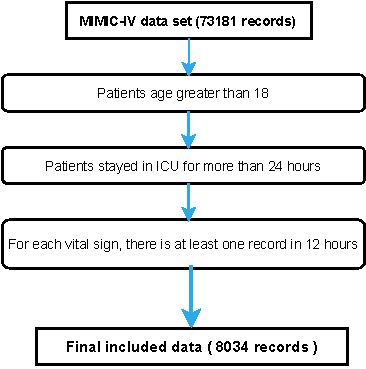
\includegraphics[width=0.8\textwidth]{thesis/img/include_criteria.pdf}
  \end{center}
  \caption[Inclusion Criteria]{Inclusion Data Criteria}
  \label{fig:include_criteria}
\end{figure*}

\section{Feature Reduction}
When training a machine learning model, there are commonly too much features collected in dataset. However, not all of them are needed. Only those features with higher correlation with target would be used in training. Correlation coefficient is used to evaluate the correlation between two features or one feature and target. The features with low correlation with target will commonly be dropped off. And if two features has high correlation, one of them would be dropped off when training a model. 

Correlation coefficient is a statistical measure that expresses the linear relationship and direction of two variables, meaning that they can move together at a constant rate. It ranges from -1 to 1, where 0 means no correlation. The coefficient larger than 0 is positive correlation and lower than 0 is negative correlation. The large correlation is indicated with large absolute value of correlation coefficient. Here we will introduce two correlation coefficient

\subsection{Pearson Correlation}
Pearson correlation, denoted by "r", is a measure of relations between two continuous variables, which is commonly used in linear relationship. It means when one variable increases, another variable will increase (positive correlation) as well, or decrease (negative correlation) as well. The Pearson correlation coefficient value is the actual coefficient value. It is widely used to measure correlation of two variables. However it is very sensitive to outliers, which can potentially misleading the interpretation of the relationship. The formula of Pearson Correlation is
\begin{equation*}
  r =
  \frac{ \sum_{i=1}^{n}(x_i-\bar{x})(y_i-\bar{y}) }{%
        \sqrt{\sum_{i=1}^{n}(x_i-\bar{x})^2}\sqrt{\sum_{i=1}^{n}(y_i-\bar{y})^2}}
\end{equation*}
Besides assessing correlation, Pearson correlation also has utility in gauging ML model efficacy, where values predicted by models are compared with real values. Hence, it was used in models predicted postprandial glucose. \parencite{kirk2021} 

\subsection{Spearman Correlation}
Spearman correlation coefficient, denoted by \(\rho\), is a measure of monotonic relationship between two variables. It is suitable for ordinal or non-normally distributed data. Rather than actual coefficient value, Spearman correlation coefficient is based on the ranks of the data. It assesses the whether variables change together, a constant rate of which is not necessary. The formula of Spearman Correlation is
\begin{equation*}
    \rho = 1- {\frac {6 \sum d_i^2}{n(n^2 - 1)}}
\end{equation*}
where \textit{d} is the difference between the ranks of corresponding variables and \textit{n} is the number of data points. It is robust to outliers since it operates on ranks, instead of actual data. As the number of data points is also a parameter in the formula, it affects the precision. It act less precise with small size data than large size. Spearman correlation is commonly used when  the relationship between variables cannot be assumed to be linear.

In this research, to get a good correlation measurement, both coefficients are used to check the relationship between variables and target, LODS value.

\section{Missing Data Imputation}
In real world, data missing is a common problem in machine learning. Most classifiers do not work correctly when input data contains empty elements.
There are three types of missing data, classified by \textcite{rubin1976}
1. Missing Completely at Random (MCAR), where the probability of being missing is same for all data and does not depend on known values or the missing value itseld. It means that the causes of the missing data are not related to data. For instance, a data table was printed without missing values, but someone accidentally dropped on it, which caused some cells are not readable. The probability of each cell be dropped is same. In this situation, the missing data could be considered as following the same distribution as the known values, and many of the complexities would be ignored consequently apart from the obvious loss of information.
2. Missing at Random (MAR), where the probability of being missing is same only within the groups defined by observed data, and depends on the known values but not on value itself. MAR class contains broader than MCAR. For instance, when someone dropped 1ml ink on a printed data table and 100ml ink on the same printed table, which caused some cells are not readable. The probabilities of each cell being unreadable are different in the two situations. MAR is more general than MCAR, which causes that modern missing data methods generally start from the MAR assumption.
3. Not Missing at Random (NMAR), where the probability of being missing is unknown and depend on the value of variable itself. In NMAR, missing data likely contains potentially valuable information. For instance, a printed data table has several specific rows are are covered with ink. Then those rows are not missing at random and contain information. NMAR is the more complex than the other two cases, strategies to handle that are finding more data to figure out the causes, or performing what-if analyses to check how sensitive the results are under different scenarios. \parencite{vanbuuren2018}
\subsection{Linear Interpolation}
Linear interpolation is an method for one-dimensional data interpolation. It bases on the two data points adjacent to the target point to estimate the data value in the one-dimensional data sequence, as \ref{fig:linear_impute_fig}. With the simplest linear interpolation, the target points are joined by straight line segment. As a result, each segment is interpolated independently and segments discontinue at each point. \parencite{huang2021, paul1999}
In contrast, a smoother interpolating function is desirable. Cosine interpolation and Cubic interpolation are two simple methods.

\begin{figure*}
  \begin{center}
    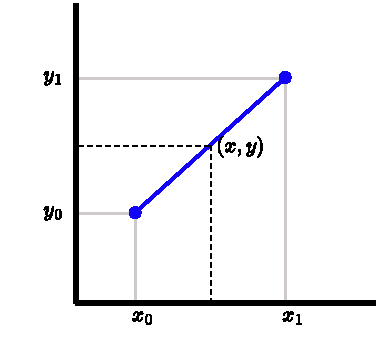
\includegraphics[width=0.7\textwidth]{thesis/img/linear_impute.pdf}
  \end{center}
  \caption[Linear Interpolation]{Linear Interpolation to calculate missing data between two known data points}
  \label{fig:linear_impute_fig}
\end{figure*}

\subsection{Probabilistic Principal Component Analysis}
Probabilistic Principal Component Analysis (PPCA) is a probabilistic extension of Principle Component Analysis (PCA). Here is an instruction of PCA and PPCA, comes from \textcite{lindsay2002} and \textcite{tipping2002}.
Principle Component Analysis, developed by Karl Pearson in 1901, is a powerful dimensionality reduction technique that aims to transform high-dimensional data to low-dimensional space without losing most of the variance in the data. \parencite{mackiewicz1993} The variables in low-dimensional space are called principle components, which are linear combinations of original variables. This is achieved by finding the directions along which the variance of the data is maximized. It is used for data compression, dimensionality reduction and data visualization. Here to explain how Principle Component Analysis works in details.

Standardization ensures that all variables are on same scale (normally 0 - 1) and prevents variables with large magnitudes from dominating the analysis, by subtracting the mean and dividing by the standard deviation of each variables. For each feature $X_i$ in the dataset, standardized value $Z_i$ should be calculated with:
\begin{equation*}
    {Z_i} = {\frac {{X_i}-{\mu_i}}{\sigma_i}}
\end{equation*}
where $\mu_i$ is the mean of feature $X_i$ and $\sigma_i$ is the standard deviation.

Covariance Matrix provides relationship info between each pair of variables. It indicates how much two variables vary together, and a positive covariance indicates two variables tend to increase or decrease together, while a negative indicates an inverse relationship. Covariance Matrix is calculated on the standardized dataset by 
\begin{equation*}
    C = \frac{1}{n}\sum\limits_{k=1}^n (\pmb x_k - \pmb m)\;(\pmb x_k - \pmb m)^T
\end{equation*}
where $n$ is the number of observations and $m$ is the mean vector of the standardized data.

Eigenvalue Decomposition, involves decomposing the covariance matrix into eigenvectors which represent the directions of maximum variance in the data, and eigenvalues which indicate the magnitude of variance along these directions. Each eigenvector correspond to a principle component, and the eigenvalue associated to is represents the amount of variance explained by that component. 

Selection of Principle Components in PCA sorts the eigenvalues in descending order and selects the top k eigenvectors (consider as principle components) that correspond to the largest eigenvalues. These principle components capture most of the variability.

Projection in PCA projects the original data onto a new orthogonal basis formed by the selected principle components. The transformation will create a new dataset where each observation is represented by a linear combination of the principle components.

However, in Probabilistic Principle Component Analysis (PPCA), the principle components are treated as random variables. The observed data is generated by a linear transformation of a lower-dimensional latent space plus Gaussian noise. The latent space is dimensionally lower than the origin data space and captures the essential features of data. Maximum likelihood estimation or Bayesian inference is used to estimate the parameters of the model, including the latent variance space and the noise variance. With the estimated parameters, the latent space can be used for dimensionality reduction. 

With a data set $X$ consisting of $N$ data points, each of dimension $D$. And the target lower-dimensional latent space $Z$ of dimension $M$ ($M$ < $D$). So, each data point $x_n$ is generated from $z_n$ through a linear transformation plus Gaussian noise:
\begin{equation*}
    {x_n} = {W}{z_n}+{\mu}+{\epsilon _n}
\end{equation*}
where $W$ is a $D$ $\times$ $M$ matrix of the loading vectors, representing the linear transformation from the latent space to the observed data space, $z_n$ is a $M$ -dimensional latent variable associated with n-th data point, $\mu$ is the mean of the data, and $\epsilon _n$ is Gaussian noise with mean zero and covariance matrix.
In PPCA, the latent variables $z_n$ are assumed to follow a Gaussian distribution:
\begin{equation*}
    {z_n} \sim {\mathcal{N}}(0, {I})
\end{equation*}
where $I$ represents the identity matrix, which is a square matrix with ones on the diagonal and zeros elsewhere. Once the $W$, $\mu$, and $\sigma ^2$ are estimated by maximizing the log-likelihood function, the latent space $Z$ (a $M$$\times$ $N$ matrix containing the latent variables for all data points) can be obtained by:
\begin{equation*}
    {Z} = {W^T}{({W}{W^T}+{\sigma ^2}{I})^{-1}}({X}-{\mu}{1^T})
\end{equation*}
where 1 is a column vector of ones.

To impute the missing data $x_{ij}$ in the observed data matrix $X$, the first step is to estimate the corresponding latent variable $z_{ij}$ with the estimated loading matrix $W$ and the latent space $Z$. Then reconstructing the missing entry  $x_{ij}$ can be done by
\begin{equation*}
    {x_{ij}} = {W_j}{z_{ij}}+{\mu _j}
\end{equation*}
where $W_j$ is the $j$ -th column of $W$ and $\mu_j$ is the $j$-th element of the mean vector $\mu$.


\section{Models}
\subsection{XGBoost}
Decision trees are powerful non-parametric classifiers and regressors which produce a recursive binary partitioning of the feature space. They build a flowchart-like tree structure where nodes represents features, branches represents decisions and leaf node represents the outcomes. When classifying new instances, decision tree locates the area where the instances lies and take a majority vote inside the area to determine the result, based on the training set, which results it low bias and high variance. XGBoost is an ensemble of decision trees using gradient boosting. In the following, we will examine how XGBoost actually works, according to \textcite{song2015, chen2016, mitchell2017, hastie2009,analytics_xgboost,stanford_ml, geek_xgboost}

Start with decision trees. Each tree is constructed by splitting the training data into subsets recursively based on attribute selection measures until the tree met a stopping criteria, such as the depth of a tree. Attribute selection measure (ASM) is used to evaluate the usefulness of different attributes for splitting a dataset, the goal of which is to determine the best attribute that will create the most homogeneous subset of data after splitting, thereby maximizing the information gain. This process is repeated in a recursive manner, called recursive partitioning, on each derived subset. When the subset at a node all has the same target value or when splitting does not add value, the recursion is completed. There are several commonly used attribute selection measures:

Entropy, is the measure of the uncertainty or randomness in a set of elements, based on the distribution of class labels in the dataset. Entropy of each classified subset ${D}$ is calculated as
\begin{equation*}
    Entroy(D)=-\sum_{i = 1}^C {p_i} \log _2 {p_i}
\end{equation*}
where ${p_i}$ is the proportion of the data points that belong to class ${i}$ in subset ${D}$ , and ${C}$ is the number of classes. ${p_i}$ is calculated with
\begin{equation*}
    p_i = \frac{1}{n} \sum I(y=i)
\end{equation*}
where ${n}$ is the amount of data points in subset.
A high entropy indicates a high maximum uncertainty. Therefore, the even distribution of class labels has the highest entropy. In contrast, low entropy indicates low randomness of the dataset. So, a completely homogeneous dataset has entropy value 0. Entropy is used to evaluate the the quality of a split, whose goal is to select attribute that minimizes the entropy of the resulting subset.

Gini Impurity, measures the probability of incorrectly classifying a randomly chosen element if it was randomly labeled according to the distribution of class labels. It is calculated as 
\begin{equation*}
    Gini(D) = 1-\sum_{i=1}^C {p_i}^2
\end{equation*}
where ${p_i}$ is the proportion of the data points classified as ${i}$ in subset ${D}$, and ${C}$ is the number of classes. A lower Gini Impurity indicates more homogeneous, that a subset is predominately composed of data points belonging to same class, than a higher one. Moreover, information gain is also a commonly used measurement in decision tree algorithm of the reduction in entropy results from a split.

Decision tree analyses the data set to predict its classification. It commences from the root node, the topmost node and starting point in a tree, where the algorithm compares the value of the root attribute and the attribute of the record in the actual data set. Then the algorithm proceeds to follow the branch and move to the next node. It repeats this action on each subsequent node until the leaf nodes of the tree. In each node, the algorithm finds the best attribute in the dataset with attribute selection measure. The total time of training a decision tree, include training and test is ${O_{(ndf)}}$, where ${n}$ is the amount of examples, ${f}$ is the feature amount and ${d}$ is the depth of the tree. 
Decision trees are simple to understand as it follows the same process as a human makes decisions in real-life. \ref{fig:decision_tree} shows an example of decision tree structure. Also, no domain knowledge or parameter setting is required to construct a decision tree, therefore it is appropriate for exploratory knowledge discovery. As its calculation focuses on the outcome of each split instead of the inputted features and it commonly process one attribute in each node, it can handle high-dimensional data. But a decision tree may have over-fitting issue due to its inherent nature of complex and highly branching structure to fit training data closely, especially with limited data and deep trees without depth limit, which memorize noise and outliers in the training data and grow until it perfectly fit the training data. Moreover, decision trees are sensitive to small variations in the training data, which causes decision trees are prone to high variance.

\begin{figure*}
  \begin{center}
    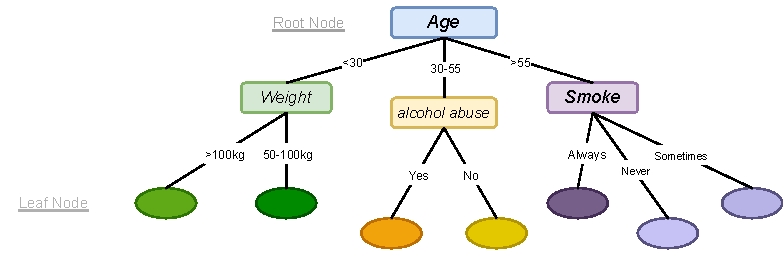
\includegraphics[width=1\textwidth]{thesis/img/decision_tree.pdf}
  \end{center}
  \caption[Decision Tree]{An example of Decision Tree Structure}
  \label{fig:decision_tree}
\end{figure*}

To address some limitations of individual decision trees and improve the overall performance of a model, ensemble decision trees is created. Bagging and boosting are two common ensemble methods. Bagging ensembles decision trees that are trained in parallel on random subsets of the original dataset and then aggregates their individual results, by voting for classification tasks or averaging for regression tasks, to form a final result. This means that some instances may be repeatedly selected, however, some may be not selected at all, which introduces further randomness and decorrelation between trees. Also with the random selection of instances, the probability of overfitting is minimized and the stability is increased as the impact of outliers and noise are reduced. Random forest is a common used powerful tool based on bagging.

Boosting is an iterative ensemble learning technique where decision trees are sequentially trained to correct the errors from previous trees. In each iteration, the new tree focuses on the instances that are misclassified or have high residuals by the previous trees and assigns those instances higher weights to emphasize their importance, while the correctly classified instances receive lower weights. This adaptive weighting scheme lets boosting to focus on the most challenging instances, gradually improving the overall performance of the ensemble. When combining predictions, boosting commonly uses weighted averaging, where the predictions of each decision tree are weighted by its performance during training, in regression task. Alternatively, in classification tasks, boosting uses a weighted majority vote where the weight of each tree depends on its accuracy in training. And it also has the advantages, as bagging, that minimizing the probability of overfitting and increasing the stability. Gradient boosting, derived from boosting, builds the ensemble sequentially by training each decision tree with the residuals of the previous tree's predictions. It optimizes a loss function by minimizing the errors of the ensemble on the training data. Regularization is also applied in boosting algorithm to prevent overfitting. XGBoost is based on gradient boosting, which ensembles regression trees, a type of decision tree used for regression tasks.

Here we will explain mathematics theory of XGBoost. For a given data set with $m$ features and $n$ examples $D = \{(x_i, y_i)\}(|D|=n, x_i \in \mathbb{R}^m, y_i \in \mathbb{R})$ , the prediction is sum of each tree, in the form
\begin{equation*}
    \hat{y}_i=\phi\left(\mathbf{x}_i\right)=\sum_{k=1}^K f_k\left(\mathbf{x}_i\right), \quad f_k \in \mathcal{F}
\end{equation*}
where $K$ is the amount of trees, and $\mathcal{F}=\left\{f(\mathbf{x})=w_{q(\mathbf{x})}\right\}\left(q: \mathbb{R}^m \rightarrow T, w \in \mathbb{R}^T\right)$ is the space of regression trees. Here, $T$ is the number of leaves in a tree and $q$ represents the structure of the tree. $f_k$ represents each independent tree structure $q$ and leaf weights $w$, then the weight of $i$-th leaf is represented with $w_i$. The objective is to minimized the following
\begin{equation*}
    \begin{gathered}
\mathcal{L}(\phi)=\sum_i l\left(\hat{y}_i, y_i\right)+\sum_k \Omega\left(f_k\right) \\
\text { where } \Omega(f)=\gamma T+\frac{1}{2} \lambda\|w\|^2
\end{gathered}
\end{equation*}
where $l$ is the loss function that measures the difference between the target $y_i$ and the prediction $\hat{y_i}$. The second part $\Omega$ is the regularization parameter, that is used to smooth the final learnt weights, to avoid over-fitting. Instead of learning all trees at once, the additive strategy is applied here to minimize the loss, summarised as below:
\begin{equation*}
    \begin{aligned}
& \hat{y}_i^{(0)}=0 \\
& \hat{y}_i^{(1)}=f_1\left(x_i\right)=\hat{y}_i^{(0)}+f_1\left(\mathbf{x}_i\right) \\
& \hat{y}_i^{(2)}=f_1\left(\mathbf{x}_i\right)+f_2\left(\mathbf{x}_i\right)=\hat{y}_i^{(1)}+f_2\left(\mathbf{x}_i\right) \\
& \cdots \\
& \hat{y}_i^{(i)}=\sum_{k=1}^i f_k\left(\mathbf{x}_i\right)=\hat{y}_i^{(t-1)}+f_i\left(\mathbf{x}_i\right)
\end{aligned}
\end{equation*}
Then, combine this to the objective function and apply taylor series expansion, the objective function will be:
\begin{equation*}
    \mathcal{L}(\phi)=\sum_{i=1}^n\left[l\left(y_i, \hat{y}_i^{(t-1)}\right)+q_i f_i\left(x_i\right)+\frac{1}{2} h_i f_i^2\left(x_i\right)\right]+\Omega\left(f_i\right)
\end{equation*}

where $g_i=\partial_{\hat{y}^{(t-1)}} l\left(y_i, \hat{y}^{(t-1)}\right)$ and $h_i=\partial_{\hat{y}^{(t-1)}}^2 l\left(y_i, \hat{y}^{(t-1)}\right)$. Then apply the regularization term which is defined earlier, the objective function becomes:
\begin{equation*}
    \begin{aligned}
& \mathcal{L}(\phi) \approx \sum_{i=1}^n\left[g_i w_{q\left\{w_j\right)}+\frac{1}{2} h_i w_{q\left(i_i\right)}^2\right]+\gamma T+\frac{1}{2} \lambda \sum_{j=1}^T w_{i j}^2 \\
= & \sum_{j=1}^T\left[\left(\sum_{i \in I_j} g_i\right) w_j+\frac{1}{2}\left(\sum_{i \in I_j} h_i+\lambda\right) w_j^2\right]+\gamma T \\
= & \sum_{j=1}^T\left[G_j w_j+\frac{1}{2}\left(H_j+\lambda\right) w_j^2\right]+\gamma T
\end{aligned}
\end{equation*}
where $G_j=\sum_{i \in I_j} g_i $ and $H_j=\sum_{i \in I_j} h_i$. The $w_j$ are independent of each other, the optimal weight $w_j^*$ of a fixed tree is
\begin{equation*}
w_j^*=-\frac{G_j}{H_j+\lambda}
\end{equation*}
and the corresponding optimal value is calculated by
\begin{equation*}
\mathcal{L}(\phi)=-\frac{1}{2} \sum_{j=1}^T \frac{G_j^2}{H_j+\lambda}+\gamma T
\end{equation*}


\subsection{Convolutional Neural Networks}
All the aforementioned models have a simple two-layer architecture of the form input directly to output. However, there is a subset of machine learning, called deep learning, that uses multi-layer neural network to mimic the complex decision-making process of human brain. Neural networks make up the backbone of deep learning. Here we will start from neural network, according to \textcite{stanford_ml, stanford_cnn, xinyu2019, yamashita2018, veena2024}. 

\begin{figure*}
  \begin{center}
    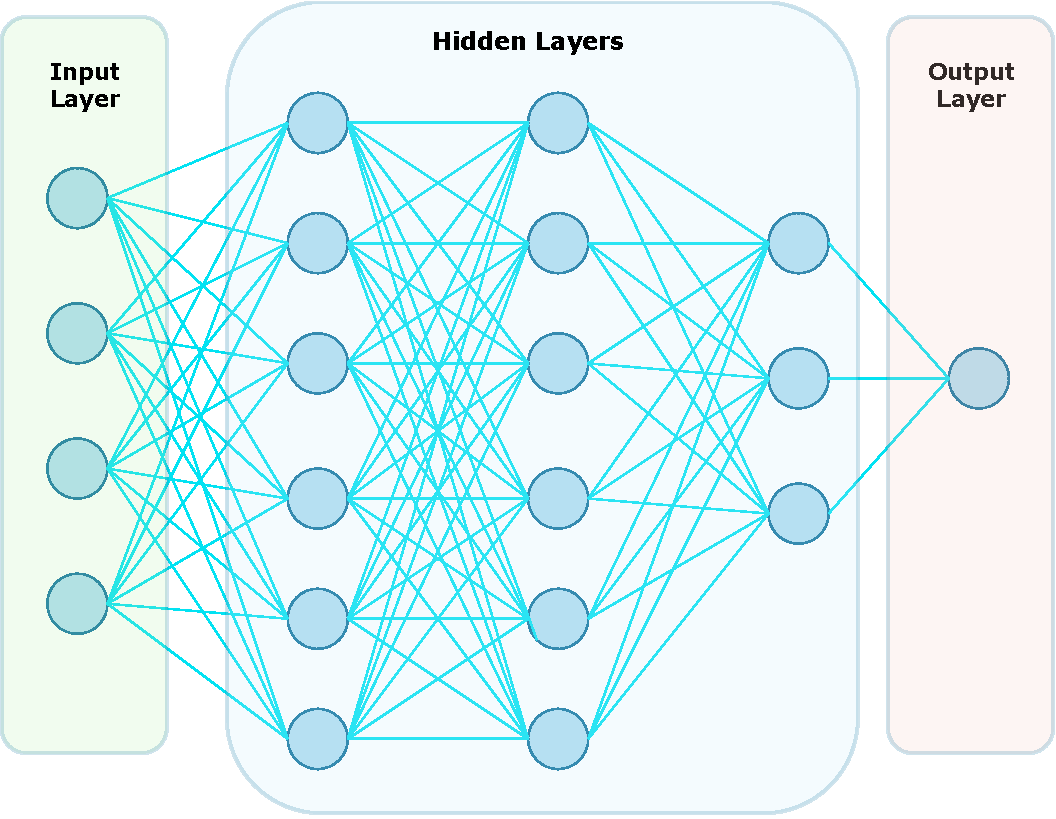
\includegraphics[width=1\textwidth]{thesis/img/neural_network.pdf}
  \end{center}
  \caption[Neural Network]{Neural Network Structure}
  \label{fig:neural_network}
\end{figure*}

Inspired by the structure and function of the brain, a neural network is a computational model that consists of  interconnected nodes or neurons, which are mathematical functions that perform a computation based on inputs and produce an output, in a layered structure. The layers between input and output layers are referred as hidden layers. Neurons inside each layer are not connected, but connected with neurons in subsequent layer through weighted connections. Each connection has an associated weight that determines the strength of the connection, as \ref{fig:neural_network}. The first step to start a basic feedforward neural network is initialization, where the weights $W$ are initialized randomly and bias $b$ are initialized to zeros. The second step is forward propagation, which passes the input data through each layer of the network, performs computations and produce an output. After data is inputted, the weighted sum of inputs for each neuron is computed in the hidden layers and output layer with
\begin{equation*}
    z^{(l)}=W^{(l)} \cdot a^{(l-1)}+b^{(l)}
\end{equation*}
where $z^{(l)}$ is the weighted sum of inputs for layer $l$, $W^{(l)}$ is the weight matrix for layer $l$, $a^{(l-1)}$ is the output of the previous layer and $b^{(l)}$ is the bias vector for layer $l$. An activation function applies to the weighted sum $z^{(l)}$ to get an output of each neuron:
\begin{equation*}
    a^{(l)}=\sigma\left(z^{(l)}\right)
\end{equation*}
The most common activation functions are reLU, sigmoid, tanh and softmax. They are used depending on the type of layer and task. In this study, we used reLU. Applying an activation function will introduce non-linearity into the network, which can capture complex patterns as the real-world datasets exhibit complex relationships that can not be modeled only by linear functions, and break symmetry in the network to prevent all neurons from learning the same representation. This process will be applied on each neuron of each hidden layer and output layer, and produce a predicted result $\hat{y}$ to compute loss between it and the actual $y$ with loss function $L(\hat{y}, y)$, which is the third step. One commonly used loss function is Mean Squared Error:
\begin{equation*}
    M S E=\frac{1}{n} \sum_{i=1}^n\left(y_i-\hat{y}_i\right)^2
\end{equation*}
where $n$ is the amount of examples. The objective is to minimize the loss. To archive this, backpropagation is applied by adjusting the weights and biases, typically with gradient descent. It starts from the output layer to compute the gradient of the loss:
\begin{equation*}
    \delta^{(L)}=\frac{\partial L}{\partial a^{(L)}} \cdot \sigma^{\prime}\left(z^{(L)}\right)
\end{equation*}
where $\frac{\partial L}{\partial a^{(L)}}$ is the gradient of loss function with respect to the activations, $\sigma^{\prime}$ is the derivative of the activation function, and $z^{(L)}$ is the weighted sum of inputs to the output layer. The same process is propagated through each layer to compute the gradient of the loss function with respect to the activations of the previous layer and the parameters of the current layer:
\begin{equation*}
    \begin{aligned}
& \delta^{(l)}=\left(\left(W^{(l+1)}\right)^T \cdot \delta^{(l+1)}\right) \cdot \sigma^{\prime}\left(z^{(l)}\right) \\
& \frac{\partial L}{\partial W^{(l)}}=\delta^{(l)} \cdot\left(a^{(l-1)}\right)^T \\
& \frac{\partial L}{\partial b^{(l)}}=\delta^{(l)}
\end{aligned}
\end{equation*}
where $\delta^{(l)}$ is the loss gradient at layer $l$. Then gradient descent is used to update parameters:
\begin{equation*}
    \begin{aligned}
& W^{(l)}=W^{(l)}-\alpha \frac{\partial L}{\partial W^{(l)}} \\
& b^{(l)}=b^{(l)}-\alpha \frac{\partial L}{\partial b^{(l)}}
\end{aligned}
\end{equation*}
where $\alpha$ is the learning rate. The whole process, include forward propagation, backpropagation, and parameter update, is iterated to decide final parameters which produce the minimum loss and output.

Convolutional Neural Network (CNN) is the extended version of feed forward neural network primarily used for analyzing visual imagery, and predominantly used to extract the feature from the grid-like matrix dataset, such as time-series data. It is designed to learn spatial hierarchies of features automatically and adaptively from input. CNN have achieved a state-of-the-art performance on a wide range of image and grid-like matrix related tasks. It consists of multiple layers, like input layer, convolutional layer which applies filters, pooling layer which reduce computation and fully connected layers which makes the final prediction. Here's a detailed breakdown of CNN layes with time-series data.

Convolutional layer is the basic block of a CNN. It slides a filter over the input data and computes a result between the filter and the small range of the input data, with formula:
\begin{equation*}
    (I * K)(i, j)=\sum_m \sum_n I(i+m, j+n) \cdot K(m, n)
\end{equation*}
where $I$ is the input data which is commonly more than 1 dimension, $K$ is the filter, $(i, j)$ are the spatial coordinates of the feature map, and $(m, n)$ are the indices used for convolution operation. Here is an example of how convolution works. Here is an example of convolution in \ref{fig:convolution}.

\begin{figure*}
  \begin{center}
    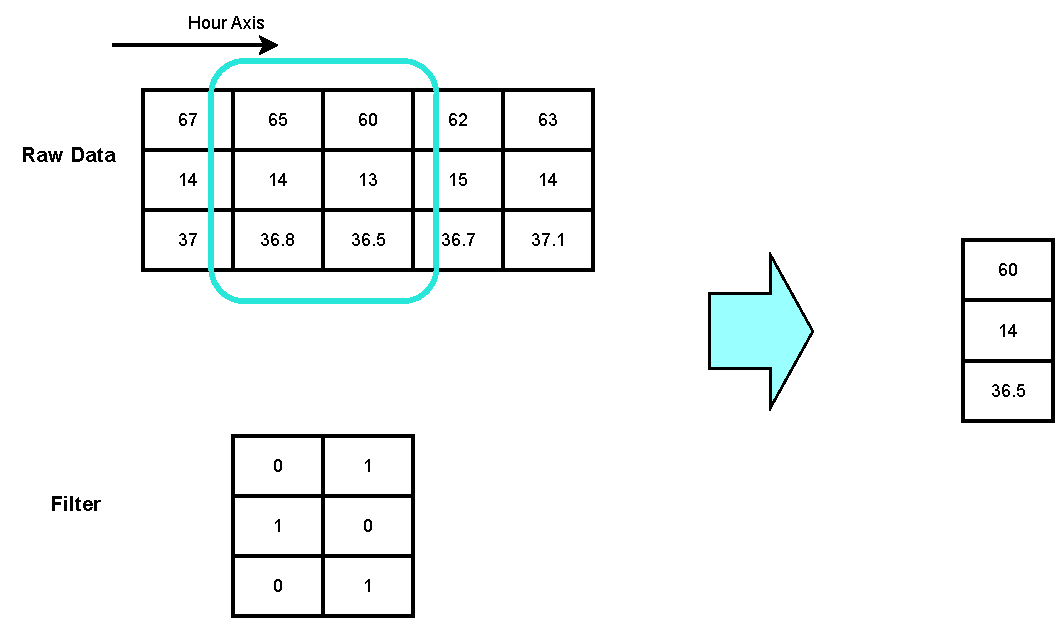
\includegraphics[width=1\textwidth]{thesis/img/convolution.pdf}
  \end{center}
  \caption[Convolution]{An example of Convolution Calculation}
  \label{fig:convolution}
\end{figure*}

Activation function is applied on the new data produced from convolution element-wise to introduce non-linearity into the network as the normal neural network.

Pooling layer is used to reduce the computational complexity and the number of parameters in the neural network, and also prevent overfitting. It is periodically inserted in the CNN. One commonly used technique is MaxPooling where the maximum value within a small window is taken as the output:
\begin{equation*}
    \operatorname{MaxPooling}(i, j)=\max \{I(i+m, j+n)\}
\end{equation*}
\ref{fig:maxpooling} is an example of MaxPooling

\begin{figure*}
  \begin{center}
    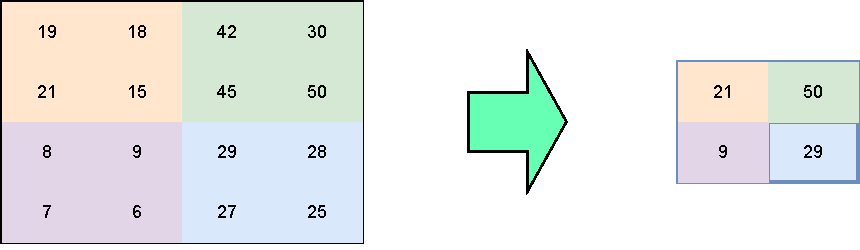
\includegraphics[width=0.8\textwidth]{thesis/img/maxpooling.pdf}
  \end{center}
  \caption[MaxPooling]{An example of MaxPooling}
  \label{fig:maxpooling}
\end{figure*}

Fully connected layer is used after several convolutional and pooling layers to perform the classification or regression task on the learned features, which is flattened into a vector. The output of a fully connected layer is fed into a logistic function, softmax or sigmoid, to obtain class probabilities in classification tasks. As neural network, loss function and backpropgation are also used in CNN to optimize the parameters.


\section{Evaluation}
Two measurements are used to evaluate the result, Mean Absolute Error (MAE) and Root Mean Square Error (RMSE). Both are common used metrics to evaluate a regression model.

Mean Absolute Error (MAE) measures the average absolute difference between the predicted values and the actual values, calculated with: 
\begin{equation*}
    \mathrm{MAE}=\frac{1}{n} \sum_{i=1}^n\left|y_i-\hat{y}_i\right|
\end{equation*}
where $n$ is the amount of observations, $y_i$ represents the actual value for observation $i$, and $\hat{y}_i$ represents the predicted value for observation $i$. MAE is robust to outliers since it considers the absolute differences. It gives equal weight to all errors, regardless of their magnitude. A low MAE indicates the absolute errors between actual values and predicted values are small, and as higher accuracy. It suggests that the model's predictions are close to the actual values, without direction of the errors. On the other hand, a high MAE indicates a poorer performance with higher prediction errors.

Root Mean Square Error (RMSE) measures the square root of the average of the squared differences between the predicted values and the actual values, calculated with: 
\begin{equation*}
    \mathrm{RMSE}=\sqrt{\frac{1}{n} \sum_{i=1}^n\left(y_i-\hat{y}_i\right)^2}
\end{equation*}
where $n$ is the amount of observations, $y_i$ represents the actual value for observation $i$, and $\hat{y}_i$ represents the predicted value for observation $i$. RMSE penalizes larger errors more heavily than smaller ones due to the squaring operation. It is sensitive to outliers because of this squaring. A low RMSE indicates the average magnitude of errors between predicted values and actual values is small, which means that the model's predictions are generally close to the actual values, as a good performance. On the other hand, a high RMSE indicates poorer performance. There is also another measurement used in this study, Mean Square Error (MSE), which is squared RMSE. It has same properties as RMSE but emphasizes larger errors due to the squaring operation.

Both MAE and RMSE are measured in the same units as the dependent variable (the variable being predicted). Lower values of both metrics indicate better model performance. MAE and RMSE are both useful metrics for evaluating the accuracy of regression models, with MAE being more robust to outliers and RMSE penalizing larger errors more heavily.


\chapter{Experiments}
\label{ch:experiment}
Computational experiments are needed to address the research questions of machine learning. Here, the goal is to specify the experiments, how they are carried out and the result. Two experiments will be introduced here, whose data preparation, feature engineering and executing will be discussed.

Two experiments were executed in this study. The aim of experiments are using bed-side data of the first 12 hours which is shorter time-range than LODS to predict the LODS, after first day stay. Experiment I uses only one value of each feature in the first 12 hours to train an model with XGBoost algorithm to finish the prediction. There is feature reduction process in the experiment whose target is to get a high performance model with small amount of features. The performance is measured with RMSE and MAE.
Experiment II uses vital sign data of each hour in the first 12 hours and several other bed-side data in the first 12 hours to predict LODS. It runs feature engineering with model trained with CNN algorithm and predicting result with a model trained by XGBoost algorithm. So in this experiment, there are two model training processes and an adjusting process which combines two models together to get a good performance. Same as experiment I, RMSE and MAE are used in this experiment as well to evaluate the performance.


After applying the inclusion criteria, there are 8034 records are used in the experiments. The amount of records of each LODS value can be found in Figure~\ref{fig:lods_distri_fig}
%\ref{table:records_amount_per_lod} 

\begin{figure}[t]
  \begin{center}
    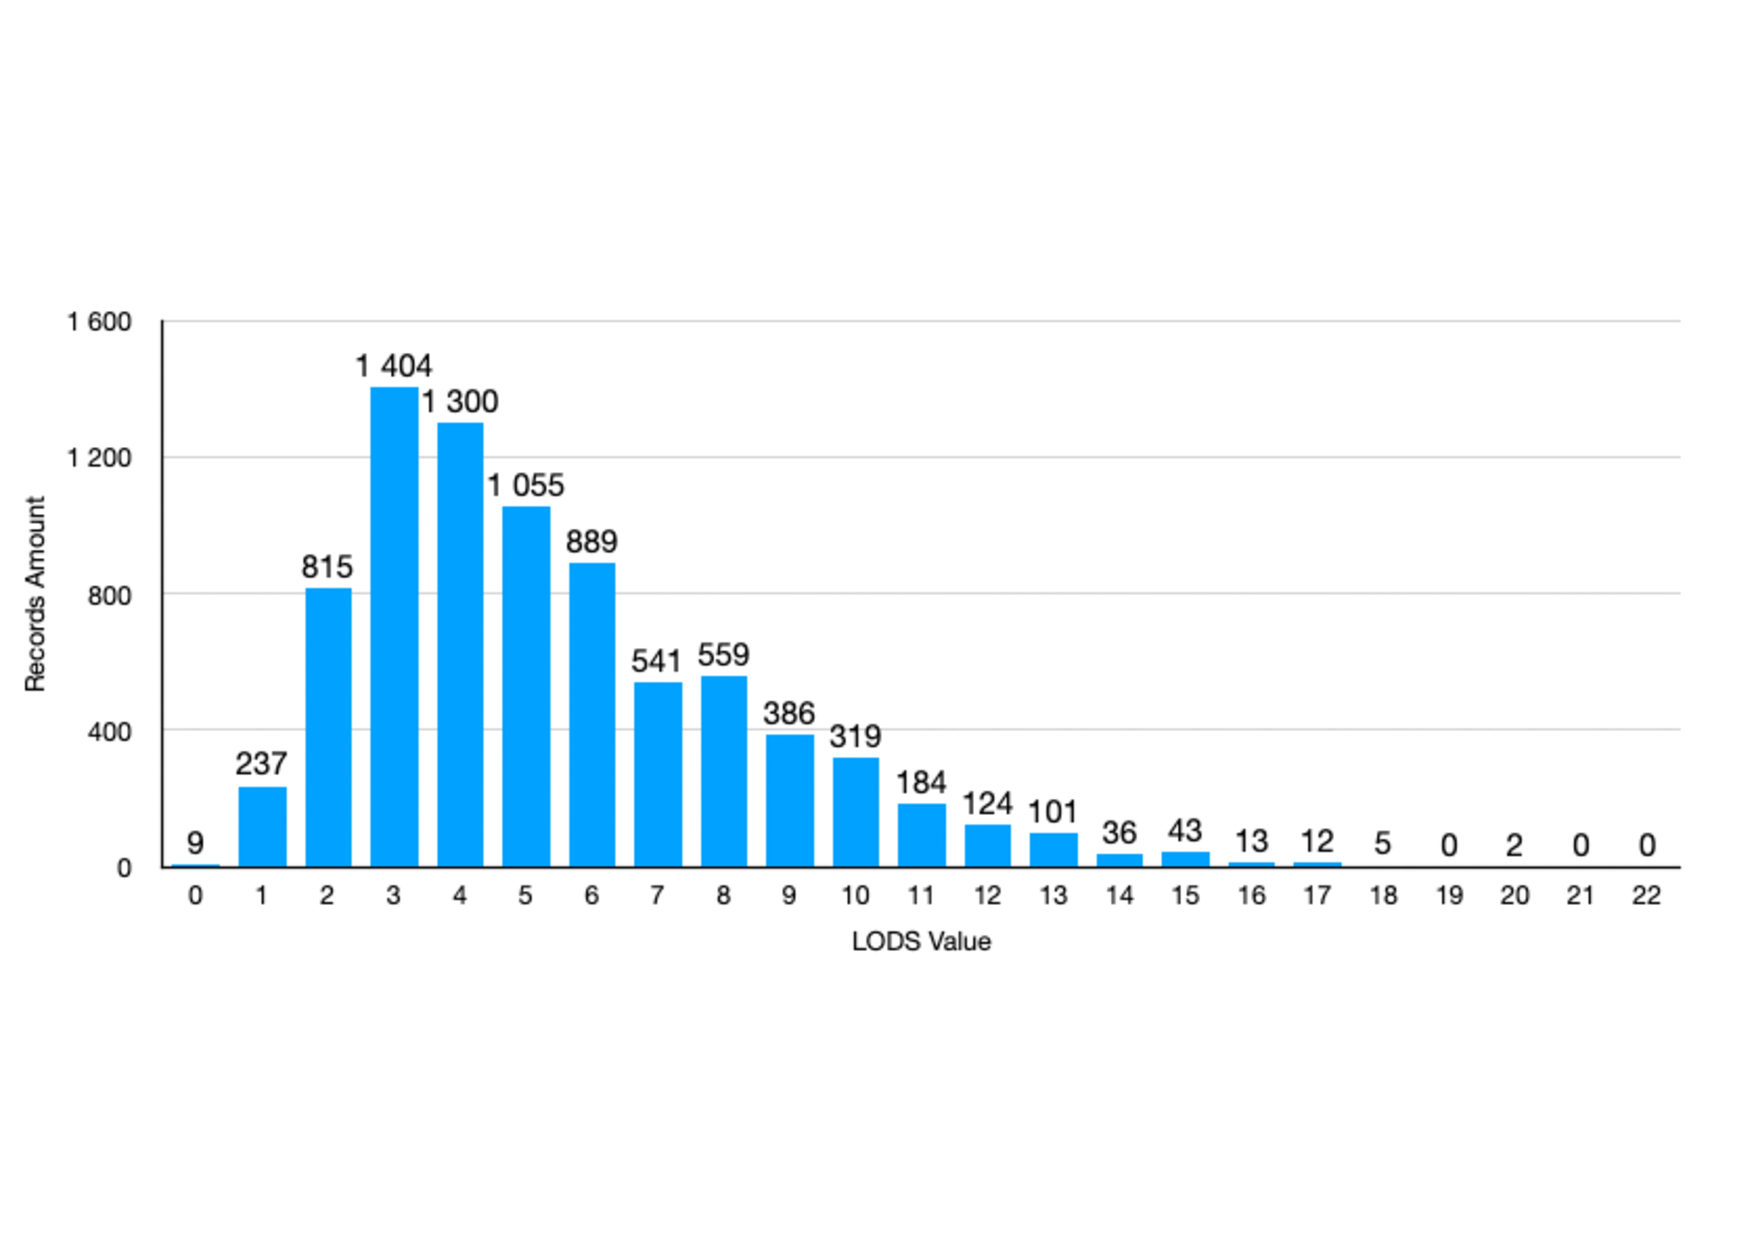
\includegraphics[width=1.0\textwidth]{thesis/img/lods_record_distribution.pdf}
  \end{center}
  \caption[Record amount of each lods value]{Records amount distribution of each LODS value}
  \label{fig:lods_distri_fig}
\end{figure}


\begin{comment}
\begin{table}[]
\centering
    \caption{Records amount per LODS value}
    \label{table:records_amount_per_lod}
    \begin{tabular}{|l|l|}
    \hline
        \textbf{LODS Value} & \textbf{Amount} \\ \hline
        0 & 9 \\ \hline
        1 & 237 \\ \hline
        2 & 815 \\ \hline
        3 & 1404 \\ \hline
        4 & 1300 \\ \hline
        5 & 1055 \\ \hline
        6 & 889 \\ \hline
        7 & 541 \\ \hline
        8 & 559 \\ \hline
        9 & 386 \\ \hline
        10 & 319 \\ \hline
        11 & 184 \\ \hline
        12 & 124 \\ \hline
        13 & 101 \\ \hline
        14 & 36 \\ \hline
        15 & 43 \\ \hline
        16 & 13 \\ \hline
        17 & 12 \\ \hline
        18 & 5 \\ \hline
        19 & 0 \\ \hline
        20 & 2 \\ \hline
        21 & 0 \\ \hline
        22 & 0 \\ \hline
        \textbf{Total:} & 8034 \\ \hline
    \end{tabular}
\end{table}
\end{comment}

Both experiments used MacBook Air 2022, with M2 CPU, 24GB Memory. XGBoost model training uses Python XGBoost Library. PPCA was performed on Matlab with \textcite{jakob2015}. CNN models are from TensorFlow.

\section{Experiment I}

Based on research from \textcite{asuroglu2021, johnson2013}, Vital signs and Glasgow Coma Scale are commonly used bed side data in this kind of research. So, we first collected the maximum, minimum and average measurements of heart rate, respiratory rate, Systolic blood pressure(sbp), Diastolic blood pressure (dbp), mean arterial pressure (MAP), Oxygen Saturation (SPO2), and temperature in the first 12 hours of ICU stay, the worst value of GCS, GCS eye, GCS motor, GCS verbal, GCS unable, the total urine output in the first 12 hours, and the most mechanical ventilation method in the first 12 hours which is ordered in Tracheostomy, Invasive Ventilation, Non Invasive Ventilation, High-flow nasal cannula (HFNC), Supplemental Oxygen and others. When collecting data, ventilation methods are coded with 1 to 6 based on the mechanical level. Moreover, patients' age and gender are also collected, where gender are coded with 0 for Male and 1 for Female.  These 30 measurements are used as input and the target is LODS value. 

\subsection{Feature Engineering}
When reviewing the data, some patients have bad maximum and minimum values for one vital sign that might come from different record time, but the average value is in normal range, which gives one idea that the average values in this experiment can not show the real situation of patient. So the average values are discarded.

To reduce the amount of features, the worst value are collected for the vital signs, as the rules in LODS and OASIS. However, to decide the worst value, a baseline value for each vital sign is used that the absolute difference between minimum/maximum value and baseline value is calculated. The one with larger absolute difference is the worst value. 

For an adult, the normal value of each vital sign is a range. Then the baseline we use the median of the range that based on \textcite{medlineplus, johnsh, torp2023, yalemed}. We take baseline as \ref{table:baseline_value} and distinguish the worst value, for instance, if a patient has maximum heart rate as 101 and minimum heart rate as 65 in the first 12 hours, then 101 is taken as the worst value. All vital signs are checked with same way.
\begin{table}[]
\centering
    \caption{Baseline values used in experiment I}
    \label{table:baseline_value}
    \begin{tabular}{|l|l|}
        \hline
        \textbf{Measurements} & \textbf{Baseline Value}\\ \hline
            Heart Rate& 80                \\ \hline
            Systolic Blood Pressure& 120               \\ \hline
            Diastolic Blood Pressure& 80                \\ \hline
            Mean Arterial Pressure& 100               \\ \hline
            Respiratory Rate& 14\\ \hline
            Temperature& 37\\ \hline
            Oxygen Saturation& 98                \\\hline
    \end{tabular}
\end{table}

\subsection{Experiment}

After gathering data from MIMIC-IV database, all records are divided by 8:2 that 80\% for training, and 20\% for test. There are 8034 records in total, 6427 records used for training the model and 1607 records used for testing. The records for testing will only be used when the model training is done which includes both training and validation. 

Applying the two correlation coefficient to check the correlation between LODS value with each parameter and got a result as table \ref{table:cc_value} where we can find the direction of correlation (negative or positive) are same in both but the values and rankings are different. So we  decided to train models with both correlation ranking and compare the results. At this stage, sequential backward selection was applied to find the best feature set. The order is following the absolute value of correlation values from low to high, as the negative is only related to direction. At the same time, I found that GCS Motor and GCS Eyes have high correlation value, 0.7687 in Pearson. So, I kept one of them when training model with Pearson correlation, GCS Motor, because it has higher correlation value with LODS than GCS Eyes. Also, hyperparameters are modified, tree amount and tree depth, to avoid overfitting. Cross validation is also applied when training the models.

\subsection{Result}
As a result, we got a model with 8 features based on Pearson correlation, GCS, GCS Motors, Ventilation Status, SPO2, Urine output, Respiratory Rate, Heart Rate and sbp, which has the best performance. MAE 1.4173 and RMSE 1.8222 in the test dataset. With \ref{table:Perfomance_comparison} we can see the performance comparison. XGBoost models' performance are better than the others. The models that take features according to Pearson Correlation perform slightly better than these according to Spearman. \ref{fig:experiment_1_result} show the predicted value and actual value comparison of each model, where the black lines refer to the perfect situation that predicted value is same as actual value. From the figure, we can find both models perform well in LODS rang 2-5 and have similar distribution. But in LODS range 10 - 20, The model trained with XGBoost and features selected with Pearson Correlation (Hereinafter referred to as XG-Pearson) has better distribution than the model trained with XGBoost and features selected with Spearman Correlation (Hereinafter referred to as XG-Spearman), that predicted values of XG-Pearson is closer to the black line.

\begin{table}[]
\centering
    \caption{Pearson and Spearman correlation coefficient}
    \label{table:cc_value}
    \begin{tabular}{|l|l|l|}
        \hline
        \textbf{Feature} & \textbf{Pearson} & \textbf{Spearman} \\ \hline
            GCS & -0.4286 & -0.1977 \\ \hline
            GCS Motor & -0.4057 & -0.3932 \\ \hline
            GCS Eyes & -0.3645 & -0.3396 \\ \hline
            Ventilation & -0.2618 & -0.2705 \\ \hline
            SPO2 & -0.2341 & -0.1416 \\ \hline
            Urine Output & -0.2300 & -0.3154 \\ \hline
            Respiratory Rate & 0.1715 & 0.1566\\ \hline
            Heart Rate & 0.1633 & 0.1232 \\ \hline
            sbp & -0.1572 & -0.2479 \\ \hline
            dbp & -0.1109 & -0.2133 \\ \hline
            map & -0.0889 & -0.2780 \\ \hline
            Temperature & -0.0638 & -0.0067 \\ \hline
            Age & 0.0505 & 0.0705 \\ \hline
            Gender & 0.0146 & 0.0121 \\ \hline
    \end{tabular}
\end{table}


\begin{table}[]
\centering
    \caption{Performance comparison in Experiment I}
    \label{table:Perfomance_comparison}
    \begin{tabular}{|l|l|l|l|l|}
        \hline
        \textbf{Model} & \textbf{Correlation} & \textbf{Features} & \textbf{MAE} & \textbf{RMSE} \\ \hline
        \multirow{2}{*}{Linear Regression} & Spearman & 12 & 1.746 & 2.214 \\ \cline{2-5} 
         & Pearson & 13 & 1.742 & 2.207 \\ \hline
        \multirow{2}{*}{Random Forest} & Spearman & 14 & 1.434 & 1.856 \\ \cline{2-5} 
         & Pearson & 13 & 1.433 & 1.856 \\ \hline
        \multirow{2}{*}{XGBoost} & Spearman & 11& 1.427& 1.840\\ \cline{2-5} 
         & Pearson & 8 & 1.417 & 1.822 \\ \hline
    \end{tabular}
\end{table}

\begin{figure*}
  \begin{center}
    \subfigure[XGBoost with Pearson Correlation]{
      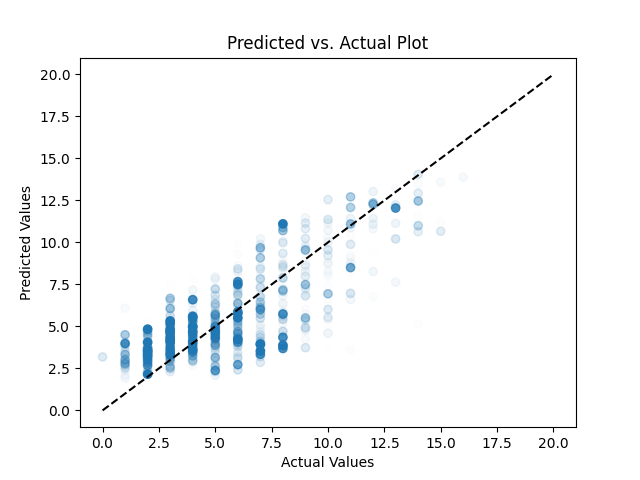
\includegraphics[width=0.45\textwidth]{thesis/img/xg_pearson.png}
      \label{subfig:xg_pearson}}
    \qquad                        
    \subfigure[XGBoost with Spearman Correlation]{
      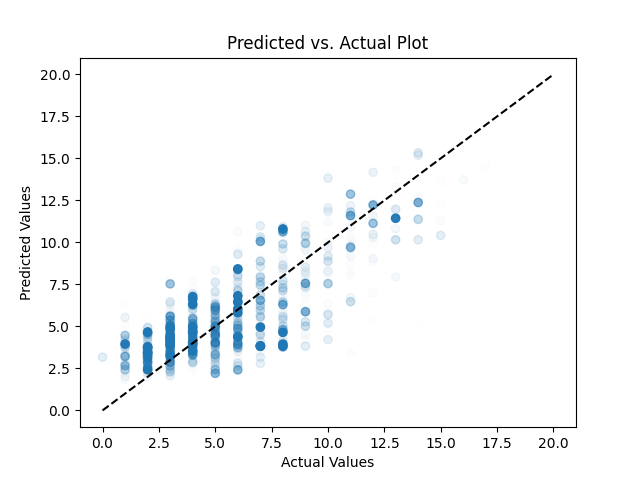
\includegraphics[width=0.45\textwidth]{thesis/img/xg_spearman.png}
      \label{subfig:xg_spearman}}
    \caption[Actual value \& Predicted value]{Comparison between actual LODS and predicted LODS in Experiment I}
    \label{fig:experiment_1_result}
  \end{center}
\end{figure*}


\section{Experiment II}

The target of Experiment II is using data of each hour in the first 12 hours to predict LODS.

In this experiment, we collected maximum, minimum and average value of vital signs of each hour in the first 12 hours, include heart rate, sbp, map, dbp, spo2, temperature, and respiratory rate. Total urine output, worst ventilation status, and worst GCS values in the first 12 hours are collected as well. The criteria is that for each vital sign, there should be at least one record in the 12 hours. Moreover, because the vital signs are monitored and recorded depends on patients' situation, not all vital signs are recorded every hour for each patient. Then there are missing data, mostly missing at random (MAR) and not missing at random (NMAR). In most situation, if a patient has recorded data in the 4 hours before move to ICU, there won't be data recorded in the first hour. So when collect data, the first hour includes the 4 hours before move into ICU and the first hour in ICU.

\subsection{Missing Data Imputation}

Two missing data imputation methods are applied in this experiment, linear imputation and PPCA. In this experiment, data missing only happens on vital signs data, where there should be 21*12 data collected. To perform the imputation, the data are listed in a 21*12 structure, ordered with time-series.

According to an interview with a medical doctor, \enquote{When checking a patient's situation, trend is more important than the exact vital sign number}. When imputing missing data, we try to keep each missing data in a trend, then linear interpolation is applied to calculate missing data. If data of the first hour or the first several hours are missing, then the first recorded data is applied on the first several hours. Same criteria applies on the last hour or the last several hours.

PPCA is performed on each records, which means each record will has its own missing data imputation process as data missing criteria varies from record to record. This process is executed with Matlab. As the data are imputed with probability calculation. There will be different value imputed for same missing data in different PPCA running processes. So the imputation was ran 5 times. Then 10 randomly selected values are compared to check the imputed result, that the criteria is that to find the better imputed results. We consider the result which is closer to the average of a total of 5 hours before and after the missing value is the better value. The 3 files with most "better imputed results" are randomly combined to create a new dataset for training.


\subsection{Feature Engineering}

In this experiment, vital signs are collected hour by hour, while the others are collected once with the worst or total value. So they are processed in different ways. Vital signs are processed with a feature engineering to extract a features from the 21*12 data. The others, total urine output, ventilation and GCS values, are proceeded without feature engineering as 1) urine output might not be an continuous operation happens in every hour or not recorded as frequent as vital signs. 2) GCS values are not recorded frequently, mostly there are less than 3 times in the first 12 hours. 3) ventilation changes very little.

With review the imputed missing data, we decided to keep the average value only with reasons: 1) patients' situation don't have large changes in one hour which means the maximum value and minimum value don't have a large gap. So it's not needed to perform the worst check as experiment I. 2) mostly there is only one value recorded in each hour, which means maximum, minimum and average are the same value. 3) To take a trend, it is either all data are maximum, or all data are minimum. But the worst value might change between maximum and minimum which will affect the trend. However, average value could show the trend. 

CNN algorithm is applied on the rest 7*12 data to extract the features. We trained models for both dataset imputed with linear imputation and PPCA. To train the model, LODS is set as target and the average vital signs of the first 12 hours are set as input. Two models are trained, best performance of each model is kept to extract data. The performance is evaluated with MSE and MAE. Then remove the last layer and take the out put as the features. (pic is needed for both models)

When training the models, we found that the MAE of both models are almost same, but the model trained with dataset imputed by PPCA has better MSE, as \ref{table:cnn_result_comparison}. This might causes from the imputed data, which let CNN model learn more details.

\begin{table}[]
\centering
    \caption{Feature engineering with CNN result comparison}
    \label{table:cnn_result_comparison}
    \begin{tabular}{|l|l|l|}
        \hline
        \textbf{Imputation Method} & \textbf{MAE} & \textbf{MSE} \\ \hline
        Linear Interpolation & 2.0494 & 6.9286 \\ \hline
        PPCA & 2.0503 & 6.8565 \\ \hline
    \end{tabular}
\end{table}

\subsection{Experiment}
The extracted features are combined with other features in model training period, include total urine output, the worst ventilation status, the worst GCS related values. According to the correlation coefficient got in Experiment I, gender and age are removed in this experiment. 

As the feature amount in a XGBoost model affects the performance, it's important to manage the feature amount. However, in CNN model, the parameter of the last layer decides the amount of outputted values. So the best way is to adjust two models together, the parameters of layers in CNN model and the hyper-parameter of XGBoost model. In CNN model, we adjust the parameters since the last layer, mainly the output amount, and one by one back the the first layer. In XGBoost model, the we adjust the amount of trees and the maximum depth of each tree to balance the amount of inputted features from CNN model, which aims to prevent overfitting and achieve the best performance. \ref{fig:xg_cnn_li_struc} show the details of model trained with XGBoost-CNN-Linear Interpolation, and \ref{fig:xg_cnn_ppca_struc} show the details of model trained with XGBoost-CNN-PPCA. They have different layers parameters.

\begin{figure*}
  \begin{center}
    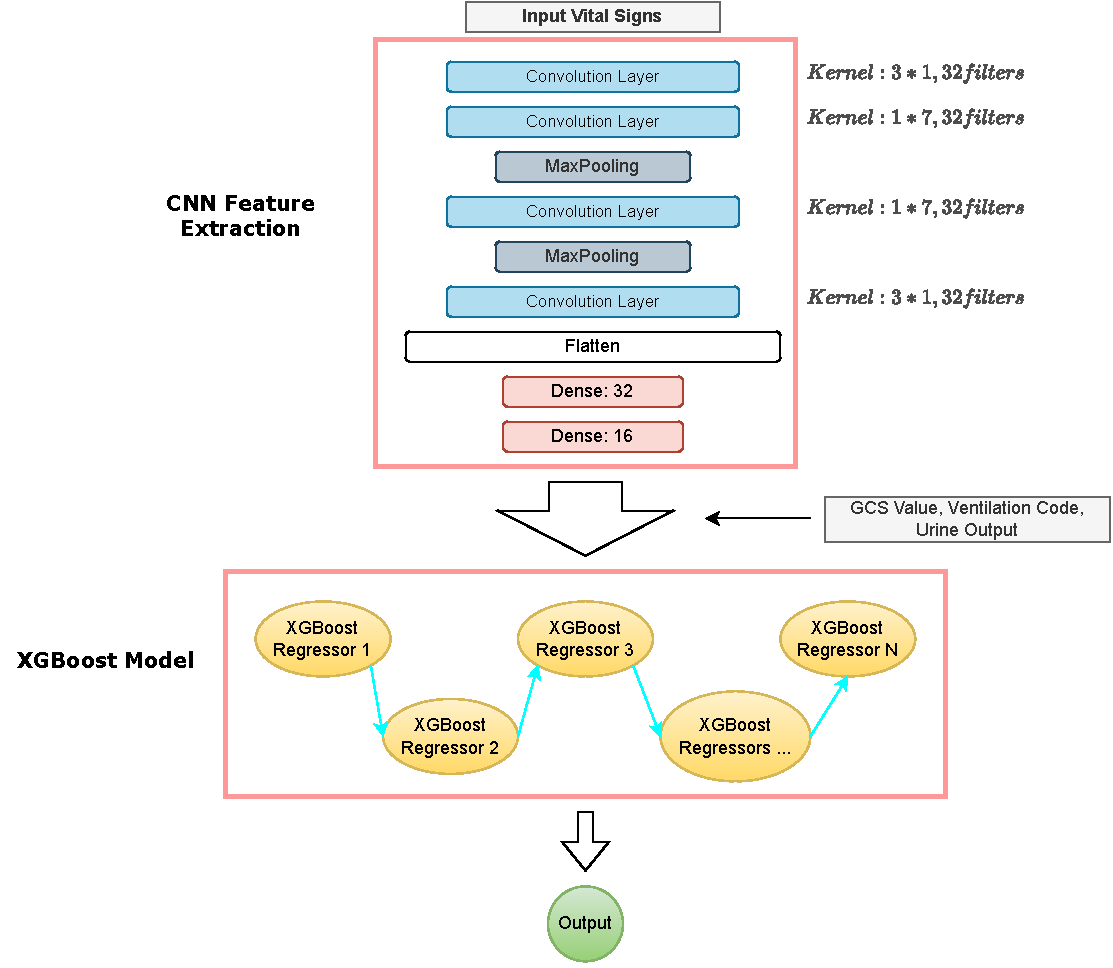
\includegraphics[width=1\textwidth]{thesis/img/xg_cnn_li.pdf}
  \end{center}
  \caption[XGBoost-CNN-LI model]{Model structure of XGBoost-CNN-Linear Interpolation}
  \label{fig:xg_cnn_li_struc}
\end{figure*}

\begin{figure*}
  \begin{center}
    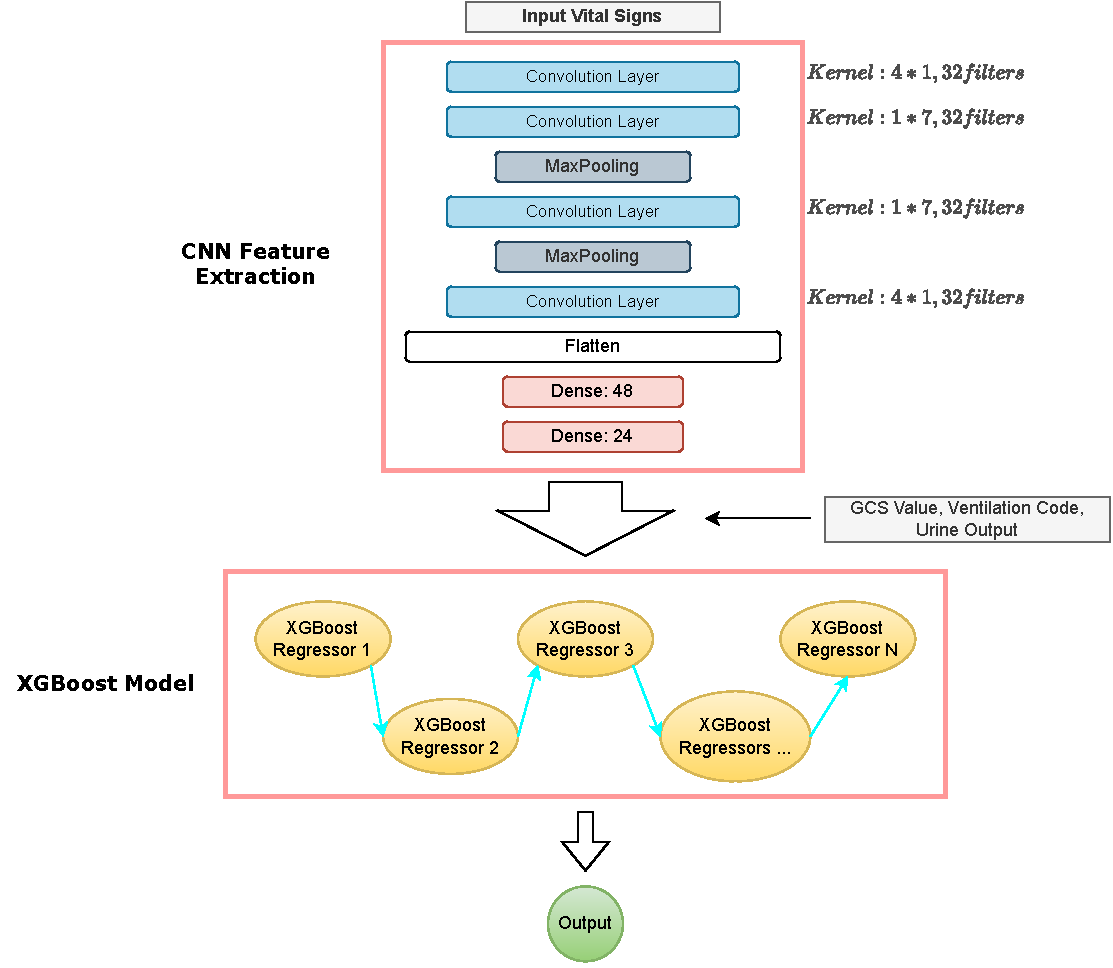
\includegraphics[width=1\textwidth]{thesis/img/xg_cnn_ppca.pdf}
  \end{center}
  \caption[XGBoost-CNN-PPCA model]{Model structure of XGBoost-CNN-PPCA}
  \label{fig:xg_cnn_ppca_struc}
\end{figure*}

\subsection{Result}
As a result, with the data imputed with linear interpolation (Hereinafter referred to as XG-CNN-LI) , we got a model that combines a CNN model of 9 layers and 16 outputs, and a XGBoost model with 100 trees, as figure. The result of the model is that RMSE is 1.912 and MAE is 1.481. With the data imputed with PPCA (Hereinafter referred to as XG-CNN-PPCA) , we got a model that combines a CNN model of 9 layers and 24 outputs and a XGBoost model with 100 trees, as figure. The result of the model is that RMSE is 1.916 and MAE is 1.468.

Compare the results of two models, performance of both models are similar. However, XG-CNN-PPCA model acts better in MAE but slightly worse on RMSE. The reason may be that it has model features input to predicting part, XGBoost training part, which causes a higher fitting level. \ref{fig:experiment_2_result} show the predicted value and actual value comparison of the two models, where the black lines refer to the perfect situation. XG-CNN-LI model performs well in predicting values range 2-5 and distributes similar in all LODS value range. When predicting values range 2 to 3, the predicted values mostly more than actual values. While predicting values range 7 to 15, the predicted values are mostly less than actual values. In contrast, XG-CNN-PPCA distributes similar in LODS ranges 1-14, only when actual value is 15, it has a bad performance. And it performs well in LODS range 2 to 6, where more values close to perfect situation.

\begin{figure*}
  \begin{center}
    \subfigure[XG-CNN-LI model comparison]{
      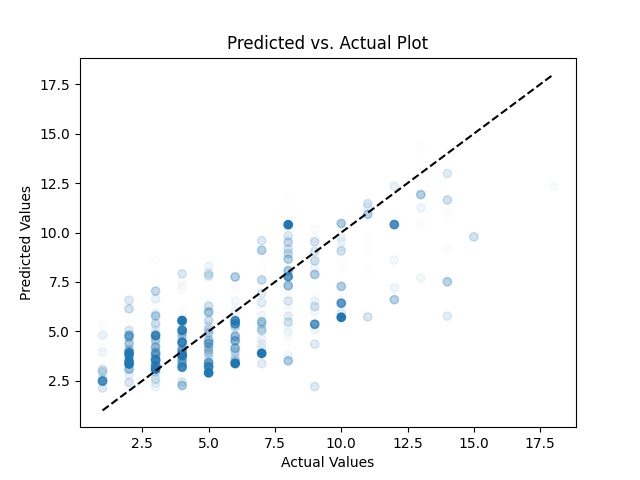
\includegraphics[width=0.45\textwidth]{thesis/img/xg_cnn_li.png}
      \label{subfig:xg_cnn_li}}
    \qquad                        
    \subfigure[XG-CNN-PPCA model comparison]{
      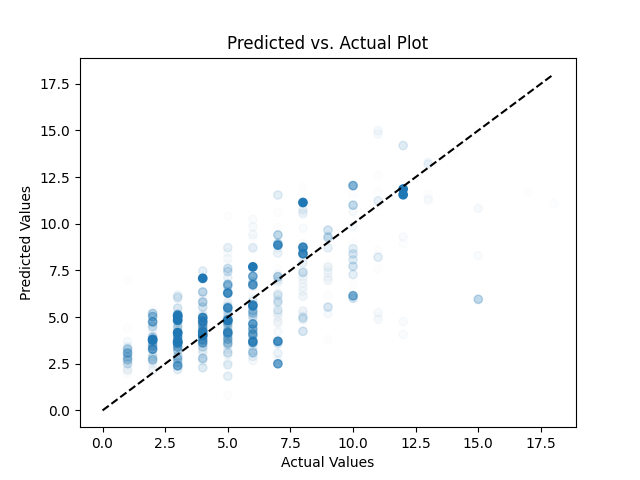
\includegraphics[width=0.45\textwidth]{thesis/img/xg_cnn_ppca.png}
      \label{subfig:xg_cnn_ppca}}
    \caption[Actual value \& Predicted value]{Comparison between actual LODS and predicted LODS in Experiment II result}

    \label{fig:experiment_2_result}
  \end{center}
\end{figure*}


\chapter{Conclusion and Discussion}
\label{ch:conclusion}
Proved in the two experiments, predicting total LODS value of first day in ICU is practicable via machine learning with first 12 hours bed-side data in ICU. With this total LODS value and original formula from LODS, patients' severity of death can be calculated. All models perform well in range LODS value 2-5, because there are many records in this range, much more than other LODS value. When considering patients' situation in this range, not a dangerous condition, the current MAE is acceptable. The model trained in Experiment I with Pearson Correlation Coefficient can be considered as a good prediction model.

But on other LODS, the performance are bad. The reason might be data for those values are too little, especially for those LODS value over 17. There are only 7 records in total 8034 records, less than 0.1\%. They might be considered as abnormal values during training. After randomly split to training set and test set, there will be less in training set, or even no records. Then even with cross validation, these records may be too little. So for further study, there should be more data in range 15 - 22 be used in training. These data need more weight as they represent a bad patient's situation. Accuracy in this range need to be higher than in range 0-5.

In Experiment I, Pearson Correlation Coefficient and Spearman Correlation Coefficient are used. Their performance are different. Pearson Correlation Coefficient worked better then Spearman Correlation Coefficient, that model with Pearson correlation uses less features and provide better prediction result than the model with Spearman correlation. Pearson correlation originally measures linear relationship between two variables. But vital signs or ventilation status shouldn't have directly linear relationship with LODS value. The connection is that some vital signs, for instance heat rate, are involved in LODS parameters, but this can not be considered as linear relationship. This experiment show a new thought, that even though features and target don't have linear relationship, Pearson Correlation Coefficient can still be used to measure correlation.

Moreover, with both correlation coefficients, GCS Motor and GCS Eyes have high correlation with LODS value. When considering these values background, we can take a wild guess that human movement condition and eye reaction condition may also represent overall organ system situation, or partly represent. 

In Experiment II, PPCA and Linear Interpolation are both applied and compared. In both feature engineering  period and XGBoost model training period, the dataset whose missing value are imputed with PPCA acts better than Linear Interpolation. Even though the difference is small, we can still get a conclusion that PPCA is a better option to perform missing data imputation than linear interpolation. Moreover, when compare results, XG-CNN-PPCA has a better distribution in all LODS ranges. It is a more promising model. It may perform much better when more data whose actual value ranges in 15 to 22 are included in training.

When compare results of experiment I and experiment II, experiment I results are better than experiment II. The feature engineering with CNN did not give better result. We can not conclude that model with XGBoost only must be better than the model with both CNN and XGBoost. The experiment II has more steps and is more complicated than experiment I. Its missing data are imputed with calculation which are different from the real data. While all the data used in experiment I are real data, which causes less uncertainties or error than experiment I. A complicated model accompanied by more uncertainties which may affect the final performance of a model. Occam's razor may also applied in model training, that the simplest model would be usually the best one.


\section{Further Research}
Data source, this research uses data from MIMIC-IV which takes medical data from Boston, Massachusetts. However, LODS was originally developed based on data from France. Due to difference in weather, diet and geographical condition, people live in these places have different body condition. So medical data from France or western Europe is another good option as data source and may train a model with better performance than the models in this study.

LODS is proved to be useful for ICU patients in the first 7 days stay. Patients' data in the first 7 days can also be included in similar study. But it should be used as a separated test set for validation, because LODS is originally designed for first 24h ICU stay.

Now, we have proved that machine learning with bed-side data can be used to predict total LODS value to show patient's organ systems situation. Bed side data and machine learning can also be brought to predicting score for each organ system. Then for each organ system, less features may needed, for instance urine output may not needed for cardiovascular as it mainly measures the situation of renal.




\newpage

\printbibliography[title=References]
\addcontentsline{toc}{chapter}{References}


%
% Appendices are optional. 
% This part is semi-ugly at the moment. Please give feedback if can
% improve it.


\appendix
\pagestyle{headings}



%
% a) Not-so-handy way, but at least it works
% 
\def\appA{APPENDIX A. Something extra} % Define the name and numbering manually
\chapter*{\appA}                       % Create chapter heading
\markboth{\appA}{\appA}                % Set page header
\addcontentsline{toc}{chapter}{\appA}  % Include this in TOC
% Note that \label does not work with unnumbered chapter

Appendices are purely optional.  All appendices must be referred to in
the body text

\def\appB{APPENDIX B. Something completely different} % Define another new command
\chapter*{\appB}                       % As above, but use \appB instead of \appA
\label{app:B}
\markboth{\appB}{\appB}                     
\addcontentsline{toc}{chapter}{\appB}  


You can append to your thesis, for example, lengthy mathematical
derivations, an important algorithm in a programming language, input
and output listings, an extract of a standard relating to your thesis,
a user manual, empirical knowledge produced while preparing the
thesis, the results of a survey, lists, pictures, drawings, maps,
complex charts (conceptual schema, circuit diagrams, structure charts)
and so on.


%
% b) The other option is to use numbered chapter and our baseline
% template report.cls numbers them as A, B... The heading and TOC do
% not include prefix 'Appendix' although the page header does.
%\chapter{name of the appendix}
%\label{app:A}                          % For cross-references



\end{document}

